\documentclass[11pt]{amsart}
%\usepackage[english]{babel}
\usepackage{appendix}
\usepackage{amsmath}
\usepackage{amsfonts}
\usepackage{amssymb}
\usepackage{dsfont}
%\usepackage{showlabels}
\usepackage{hyperref}
\usepackage{amsthm}
\usepackage{marginnote}
\usepackage{stmaryrd}
\usepackage{enumitem}
\usepackage[english]{babel}
\usepackage{yfonts}
\usepackage[T1]{fontenc}
\usepackage[utf8x]{inputenc}
%\usepackage{enumerate}
\usepackage{verbatim}
\usepackage{graphicx}
\usepackage{verbatim}
\usepackage{faktor}
\usepackage{xcolor}
\usepackage{xfrac}
\usepackage{tikz,tikz-cd}
\usetikzlibrary{decorations.pathmorphing,decorations.pathreplacing,patterns}
\usepackage[all]{xy}
\usepackage{bbm}
\usepackage{tabularx}
\usepackage{longtable}
\usepackage{tabu}
\usepackage{booktabs}
\usepackage{mathtools}

\newcommand{\TT}{\operatorname{T}}
\newcommand{\oM}{\overline{\mathcal{M}}}
\newcommand{\M}[4]{\overline{\mathcal{M}}_{#1,#2}(#3,#4)}
\newcommand{\MK}[4]{\overline{\mathcal{M}}^{\rm{Kim}}_{#1,#2}(#3,#4)}
\newcommand{\Q}[4]{\mathcal{Q}_{#1,#2}(#3,#4)}
\newcommand{\Qe}[4]{\mathcal{Q}^{\epsilon}_{#1,#2}(#3,#4)}
\newcommand{\Qt}[4]{\widetilde{\mathcal Q}_{#1,#2}(#3,#4)}
\newcommand{\QG}[4]{\mathcal{QG}_{#1,#2}(#3,#4)}
\newcommand{\QGe}[4]{\mathcal{QG}^{\epsilon}_{#1,#2}(#3,#4)}
\newcommand{\D}[3]{\mathcal{D^Q}(#1,#2,#3)}
\newcommand{\E}[3]{\mathcal{E^Q}(#1,#2,#3)}
\newcommand{\PP}{\mathbb P}
\newcommand{\QQ}{\mathbb{Q}}
\newcommand{\Z}{\mathbb{Z}}
\newcommand{\N}{\mathbb{N}}
\newcommand{\OO}{\mathcal{O}}
\renewcommand{\to}{\rightarrow}
\newcommand{\A}{\mathcal A}
\newcommand{\B}{\mathcal B}
\newcommand{\C}{\mathfrak C}
\newcommand{\F}{\mathcal F}
\newcommand{\EE}{\mathbf{E}}
\renewcommand{\L}{\mathcal L}
\newcommand{\LL}{\mathbf{L}}
\newcommand{\MM}{\mathfrak M}
\newcommand{\Aaff}{\mathbb{A}}
\newcommand{\kk}{\Bbbk}
\newcommand{\comp}{\chi}
\newcommand{\sst}{\sigma^{\operatorname{ss}}}
\newcommand{\Pic}{\operatorname{Pic}}
\newcommand{\Def}{\operatorname{Def}}
\newcommand{\Spec}{\operatorname{Spec}}
\newcommand{\Proj}{\operatorname{Proj}}
\newcommand{\Hom}{\operatorname{Hom}}
\newcommand{\Ext}{\operatorname{Ext}}
\newcommand{\val}{\operatorname{val}}
\newcommand{\Gm}{\mathbb{G}_{\text{m}}}
\newcommand{\virt}[1]{[#1]^{\operatorname{vir}}}
\newcommand{\vip}[1]{[#1]^{\operatorname{prod}}}
\newcommand{\Id}{\operatorname{Id}}
\newcommand{\CC}{\mathbb{C}}
\newcommand{\ZZ}{\mathbb{Z}}
\newcommand{\HH}{\operatorname{H}}
\newcommand{\Achow}{\operatorname{A}}
\newcommand{\pt}{\operatorname{pt}}
\newcommand{\lala}{\langle\!\langle}
\newcommand{\rara}{\rangle\!\rangle}
\newcommand{\bq}{\begin{equation}}
\newcommand{\eq}{\end{equation}}
\newcommand{\ba}{\begin{aligned}}
\newcommand{\ea}{\end{aligned}}
\newcommand{\be}{\begin{enumerate}}
\newcommand{\ee}{\end{enumerate}}
\newcommand{\bsm}{\left(\begin{smallmatrix}}
\newcommand{\esm}{\end{smallmatrix}\right)}                   
\newcommand{\bpm}{\begin{pmatrix}}
\newcommand{\epm}{\end{pmatrix}}
\newcommand{\barr}{\begin{displaymath}\begin{array}{cccc}}
\newcommand{\earr}{\end{array}\end{displaymath}}
\newcommand{\barrl}{\begin{displaymath}\begin{array}{lcl}}
\newcommand{\earrl}{\end{array}\end{displaymath}}
\newcommand{\barl}{\begin{displaymath}\begin{array}{l}}
\newcommand{\earl}{\end{array}\end{displaymath}}
\newcommand{\bxym}{ \begin{displaymath}\xymatrix }
\newcommand{\exym}{\end{displaymath}}
\newcommand{\bcd}{\begin{center}\begin{tikzcd}}
\newcommand{\ecd}{\end{tikzcd}\end{center}}
\newcommand{\R}{\operatorname{R}^{\bullet}}
%\newcommand{\sslash}{\mathbin{/\mkern-6mu/}}
\newcommand{\tr}{{\rm tr}}
\newcommand{\Isom}{\text{Isom}}
\newcommand{\pr}{\operatorname{pr}}
\newcommand{\fgt}{\operatorname{fgt}}
\newcommand{\ev}{\operatorname{ev}}
\newcommand{\codim}{\operatorname{codim}}
\newcommand{\rk}{\operatorname{rk}}
\newcommand{\vdim}{\operatorname{vdim}}
\newcommand{\Bl}{\operatorname{Bl}}
\newcommand{\ildef}[1]{\emph{#1}}
\newcommand{\om}[1]{\mathcal{#1}}
\newcommand{\h}{\operatorname{h}}
\newcommand{\vv}{\operatorname{v}}
\newcommand{\Aut}{\operatorname{Aut}}
\newcommand{\RR}{\mathbb{R}}
\newcommand{\NN}{\operatorname{N}}
\newcommand{\id}{\mathrm{id}}
\newcommand{\dvr}{\Delta}

\theoremstyle{definition}
\newtheorem{thm}{Theorem}[section]
\newtheorem{lem}[thm]{Lemma}
\newtheorem{lemma}[thm]{Lemma}
\newtheorem{prop}[thm]{Proposition}
\newtheorem{cor}[thm]{Corollary}
\newtheorem*{teo*}{Theorem}
\newtheorem{ipotesi}{ipotesi}
\newtheorem*{nota}{Nota}
\newtheorem{claim}{Claim}
\newtheorem{question}[thm]{Question}
\newtheorem{conj}[thm]{Conjecture}

\newtheorem{innercustomthm}{Theorem}
\newenvironment{customthm}[1]
  {\renewcommand\theinnercustomthm{#1}\innercustomthm}
  {\endinnercustomthm}

\theoremstyle{definition}
\newtheorem{example}[thm]{Example}
\newtheorem{ex}[thm]{Example}
\newtheorem{dfn}[thm]{Definition}
\newtheorem{definition}[thm]{Definition}
\newtheorem{aside}[thm]{Aside}
\newtheorem{rmk}[thm]{Remark}
\newtheorem{com}[thm]{Comment}
\newtheorem{num}{Number}
\newtheorem*{sketch}{Sketch}
\newtheorem*{rem}{Remark}
\newtheorem*{aside*}{Aside}
\newtheorem*{acknowledgements}{Acknowledgements}

\newcommand{\ilemph}[1]{\emph{#1}}

\setcounter{tocdepth}{1}

\newcommand{\todo}[1]{\vspace{5mm}\par \noindent
\framebox{\begin{minipage}[c]{0.95 \textwidth} \tt #1\end{minipage}} \vspace{5mm} \par}

\def\ti{-\allowhyphens}
\newcommand{\thismonth}{\ifcase\month % case 0 --- impossible!
  \or January\or February\or March\or April\or May\or June%
  \or July\or August\or September\or October\or November%
  \or December\fi}
\newcommand{\thismonthyear}{{\thismonth} {\number\year}}
\newcommand{\thisdaymonthyear}{{\number\day} {\thismonth} {\number\year}}

\usepackage[T1]{fontenc}
\usepackage{newpxtext,newpxmath}

%Dedica: A chi ha lasciato col suo passaggio una voragine nel mio cuore \\ pulsante di mancanza, \\ e a chi si sforza ogni giorno di colmarla \\ senza mai stancarsi di dare amore laddove tanto abbisogna

\title[Thesis]{Alternative compactifications in low genus Gromov-Witten theory}
\author{Luca Battistella}
\begin{document}

\maketitle
\appendixtitletocoff
\tableofcontents

\section{Review of toric varieties and quasimaps}

\subsection{Definitions} Let $N$ be a lattice with dual $M=\Hom_{\ZZ}(N,\ZZ)$, $\Sigma\subseteq N_{\RR}$ a rational polyhedral fan with associated toric variety $X_{\Sigma}$, with primitive generators $v_{\rho}$ of the rays $\rho\in\Sigma(1)$. I assume throughout this text that $X=X_{\Sigma}$ is smooth and projective (equivalently every cone is spanned by a $\Z$-basis and the support of the fan is the whole of $N_{\RR}$).

In \cite{CoxFunctor} D.A. Cox gave a beautiful description of the functor of points of a smooth toric variety, generalising the well-known equivalence between maps to the projective space $\PP^N$ and the data of a line bundle with $N+1$ sections that generate it.

Recall that the rays $\rho\in\Sigma(1)$ correspond to toric divisors $D_{\rho}$ on $X$ - which generate the Picard group -, while $M$ can be thought of as the lattice of characters of the torus $T\subseteq X$, hence giving rational functions on $X$. In the smooth case the following sequence is exact:
\begin{equation}\label{eq:toric_Pic_es} 0\to M\to \ZZ^{\Sigma(1)}\to \Pic(X)\to 0\end{equation}

\begin{thm}[Cox]
 Let $X$ be a smooth toric variety with notation as above. A morphism $f\colon C\to X$ is equivalent to the data:
 \[\left((L_\rho,u_\rho)_{\rho\in\Sigma(1)},(\varphi_m)_{m\in M}\right),\]
 where $L_\rho\in\Pic(C)$, $u_\rho\in H^0(C,L_\rho)$, and $\varphi_m\colon \bigotimes_{\rho\in\Sigma(1)}L_\rho^{\otimes \langle v_\rho, m\rangle}\simeq \OO_C$, satisfying the following conditions:
 \begin{enumerate}
\item \ilemph{nondegeneracy}: for all $x \in C$ there exists a maximal cone $\sigma \in \Sigma_{\operatorname{max}}$ with $u_\rho(x) \neq 0$ for all rays $\rho \not\subset \sigma$;
\item \ilemph{compatibility}: $\varphi_m\circ\varphi_{m'}=\varphi_{m+m'},\ \forall m,m'\in M$.
\end{enumerate}
\end{thm}

\begin{rmk}
 The isomorphisms $\varphi_m$ can be used to reduce the number of line bundles down to the Picard rank of $X$.
\end{rmk}

Based on this and on previous work of A. Marian, D. Oprea and R. Pandharipande \cite{MOP} (similar ideas had in fact already appeared in the work of Drinfeld, Morrison-Plesser, Givental, and many others), I. Ciocan-Fontanine and B. Kim introduced the following notion, which gives rise to an alternative compactification of the space of maps from smooth curves to a smooth projective toric variety, by strengthening the stability requirement and weakening the concept of map (with respect to Kontsevich's space of stable maps). For this let me fix a polarisation $\OO_X(1)$ and an expression thereof as a combination of toric line bundles $\OO_X(1)=\bigotimes_{\rho\in\Sigma(1)}\OO(D_\rho)^{\otimes \alpha_\rho}$.

\begin{definition}\cite[Definition 3.1.1]{CF-K} Let $X$ be as above. We fix the following numerical invariants: a genus $g \geq 0$, a number of marked points $n \geq 0$, an effective curve class $\beta \in \HH_2^+(X)$, and a positive rational number $\epsilon$. A \ilemph{quasimap} is given by the data
\begin{equation*} \Big((C,x_1,\ldots,x_n), (L_\rho,u_\rho)_{\rho \in \Sigma(1)}, (\varphi_m)_{m \in M}\Big) \end{equation*}
where:
\begin{enumerate}
\item $(C,x_1,\ldots,x_n)$ is a prestable curve of genus $g$ with $n$ marked points;
\item $L_\rho\in\Pic^{d_\rho}(C)$  where $d_\rho = D_\rho \cdot \beta$ and $u_\rho\in H^0(C,L_\rho)$;
\item $\varphi_m \colon \bigotimes_{\rho \in \Sigma(1)} L_\rho^{\otimes \langle v_\rho, m \rangle} \simeq \OO_C$ are isomorphisms satisfying \ilemph{compatibility} under the group structure;
\item there is an at most finite set of smooth and non-marked points $B \subseteq C$, called the \ilemph{basepoints} of the quasimap, such that \ilemph{nondegeneracy} is satisfied for all $x \in C \setminus B$.
\end{enumerate}
Furthermore a quasimap is said to be $\epsilon$-\ilemph{stable} if:
\begin{enumerate}[resume]
 \item the line bundle $ \omega_C(x_1 + \ldots + x_n)\otimes L^{\otimes \epsilon}$ is ample, where $L = \otimes_\rho L_\rho^{\otimes \alpha_\rho}$ is determined by the chosen polarisation,
 \item $\epsilon \ell(x)\leq 1$, where $\ell(x)$ is the order of the basepoint:
\[\ell(x)=\min\left\{\operatorname{ord}_x\left(\prod_{\rho\in\Sigma(1)\setminus \sigma(1)}u_\rho\right)\ |\ \sigma\in\Sigma_{\operatorname{max}}\right\}.\]
\end{enumerate}
An isomorphism between two quasimaps is given by an isomorphism $\psi\colon (C,\mathbf x)\simeq(C',\mathbf x')$ of the underlying prestable curves, together with isomorphisms of the line bundles $\lambda_\rho\colon L_\rho\simeq \psi^* L_\rho'$ preserving the sections and the trivialisations.
\end{definition}

The above definitions make sense in families over arbitrary base schemes, and therefore determine the moduli space of $\epsilon$-stable quasimaps as a cfg over $(Sch)$, denoted by $\Qe{g}{n}{X}{\beta}$, which comes with universal structures, such as a curve, markings, line bundles and sections; note in particular that, since the basepoints cannot coincide with the markings, it comes with well-defined evaluation maps $\ev\colon \Qe{g}{n}{X}{\beta}\to X^n$.

\begin{rmk}
 There is a more general notion of quasimaps when the target belongs to a certain class of GIT quotients $W\sslash G$ \cite{CFKM}; smooth toric varieties fit nicely in this framework, as they can always be described as a quotient $\Aaff^{\Sigma(1)}\sslash\Gm^r$, where $r$ is the Picard rank of $X$. In this light, quasimaps can be thought of as maps to the stack quotient $[W/G]$, such that the preimage of the unstable locus is finite and disjoint from the special points. Also, GIT quotients come with a preferred polarisation over the affine quotient $W/G$. The theory deals effectively with non-projective targets in the presence of a well-behaved torus action, and with complete intersections defined by homogeneous bundles as well.
\end{rmk}
\begin{rmk}
 The $\epsilon$-stability condition is introduced in order to interpolate between Kontsevich's stable maps (for $\epsilon\gg 0$, hence denoted by $\epsilon=\infty$) and what in the sequel I will refer to just as quasimaps (for $\epsilon\ll1$, denoted by $\epsilon=0+$). Note that in the latter case necessarily $2g-2+n \geq 0$, and there cannot be \ilemph{rational tails} by stability. In between these two extrema one should imagine that rational tails of higher and higher degree are exchanged for basepoints of order lower and lower; see \S \ref{sec:collapsing} below. Notice that the stability condition does not depend on the choice of the polarisation in the chambers $\epsilon=0+$ \cite[Lemma 3.1.3]{CF-K} and $\epsilon=\infty$.
\end{rmk}

\begin{ex}\label{ex:qm_to_pt}
 Quasimaps to a point recover Hassett's moduli space of weighted pointed curves \cite{Hassett}. In particular, to set notation, $\Q{g}{n}{\{*\}}{d}\simeq \oM_{g,n|d}/S_d$ where the first $n$-markings have weight $1$, and the last $d$ (which correspond to the basepoints) have weight $0+$ and are unordered.
\end{ex}

\subsection{Basic properties}\begin{thm}\cite[Theorems 3.2.1 and 4.0.1]{CF-K}
 $\Q{g}{n}{X}{\beta}$ is a proper and virtually smooth DM stack of finite type over $\Spec(\kk)$.
\end{thm}

Here is a brief sketch of their argument. Let me examine properness first: assume we have a stable quasimap \[\left((C_K,\mathbf x_K), (L_{i,K})_{i=1,\ldots,\rk\Pic(X)},(u_{\rho,K})_{\rho\in\Sigma(1)})\right)\] over a discretely valued field $K$, such that $C_K$ is smooth; we would like to extend it over the trait $\dvr=\Spec(R)$, where $K=\operatorname{Frac}(R)$, possibly after base-change. By semistable reduction for curves and Castelnuovo's criterion, we may find a regular model $C$ over $\dvr$ with no $(-1)$-curves. Note that we may not appeal to the properness of the relative Picard functor in order to extend the line bundles (unless we restrict to genus $0$). We exploit properness of the relative Quot functor instead: after twisting with a sufficiently ample polarisation $\OO_{C_K}(m)$ on $C_K$, we find an exact sequence
\[ 0 \to L_{i,K} \to \OO_{C_K}(m)^{\oplus N_i} \to Q_{i,K}\to 0 \]
which may be extended to the whole of $C$; up to taking double duals, $L_i$ is a line bundle for every $i$. Now the $u_\rho$ are only rational sections of the relevant line bundles. But observe that the given quasimap induces a bona fide map outside the base locus, i.e. from $C_K\setminus B_K$ to $X_K$. By normality of $C$ and properness of $X$, this can be extended to a map from $C\setminus(\overline{B_K}\cup B_0)$, where $B_0$ is a finite set of points on the central fiber; we thus get that the pullback of the toric line bundles are defined everywhere, and so are the corresponding sections (by Hartogs). By twisting back with $\OO_C(\overline{B_K})$ we obtain an extension of the quasimap we started with. There may be two (fixable) issues at this point: basepoints may coincide with nodes or markings in the central fiber, which can be resolved by blowing-up (the process terminates because the newly created rational components have nontrivial quasimap degree); finally unstable components, that are $(-2)$-curves on which the line bundles and sections are constant, may be contracted by Artin's theory and all the data descend.

As for the (dual) perfect obstruction theory, the morphism to the universal Picard stack that forgets the sections $(u_\rho)$,
\[\Q{g}{n}{X}{\beta} \to \bigtimes_{i=1}^{\rk\Pic(X)}{}_{\MM_{g,n}}\left(\mathfrak{Pic}^{d_{\rho_i}}_{g,n}\right)\]
admits a perfect obstruction theory given by $\bigoplus_{\rho\in\Sigma(1)} \operatorname R^\bullet\pi_*\mathcal L_\rho$, where $\pi\colon \mathcal C\to \Q{g}{n}{X}{\beta}$ is the universal curve and $\mathcal L_\rho$ are (linear combinations of) the universal line bundles (see also \cite{Jie, CL-pfields}). On the other hand the Euler sequence for $X$ induces an exact sequence
\[ 0\to \OO_{\mathcal C}^{\oplus\rk\Pic(X)}\to \bigoplus_{\rho\in\Sigma(1)}\mathcal L_\rho\to\mathcal F_X\to 0\]
on the universal curve, which shows that a compatible perfect obstruction theory relative to $\MM_{g,n}$ is given by $\operatorname R^\bullet\pi_*\mathcal F_X$. Notice that the latter agrees with $\operatorname R^\bullet\pi_*f^*T_X$ on the open locus of quasimaps with no basepoints (i.e. maps).

In particular $\Qe{g}{n}{X}{\beta}$ is endowed with a virtual class of the same dimension as $\virt{\M{g}{n}{X}{\beta}}$. For cohomology classes $\delta_i\in H^*(X,\QQ)$ and natural numbers $a_i,\ i=1,\ldots,n$, we may therefore define descendant $\epsilon$-quasimap invariants by:
\[\langle \tau_{a_1}(\delta_1),\ldots,\tau_{a_n}(\delta_n)\rangle^{X,\epsilon}_{g,n,\beta}=\int_{\virt{\Qe{g}{n}{X}{\beta}}}\prod_{i=1}^n \ev_i^*(\delta_i)\psi_i^{a_i}.\]

\subsection{The collapsing morphism}\label{sec:collapsing} I shall start this section with an example.
\begin{ex}\label{ex:lines_in_p2}
 Consider the evaluation map $\ev\colon \M{0}{2}{\PP^2}{1}\to \PP^2\times\PP^2$: when the two image points are distinct, the map must necessarily parametrise the line between them, while when they coincide we are left with choosing a line through that point. This shows that $\M{0}{2}{\PP^2}{1}\simeq \Bl_{\Delta}\PP^2\times\PP^2$, and $\ev$ is the blow-down map. In fact the exceptional divisor consist of maps with a rational tail of degree $1$, and a $3$-pointed $\PP^1$ mapping to a point. On the other hand $\ev\colon \Q{0}{2}{\PP^2}{1}\simeq \PP^2\times\PP^2$. The modular interpretation of the blow-down map is that it collapses rational tails to basepoints. This is in fact a general feature of quasimaps to projective space.
\end{ex}

\begin{lem}
 There is a birational \ilemph{collapsing} morphism $\chi\colon \M{0}{n}{\PP^N}{d}\to \Q{0}{n}{\PP^N}{d}$.
\end{lem}

The idea is to find a line bundle on the universal curve that will give us the contraction $q\colon\mathcal C\to\hat{\mathcal C}$: if we work over $\mathfrak{Pic}^d_{0,n}=\MM_{0,n}^{\rm{wt}=d}$, the locus $\mathfrak T^\delta$ spanned by rational tails (trees) of (total) degree $\delta$ is a Cartier divisor in the universal curve $\mathfrak C\to\mathfrak{Pic}^d_{0,n}$. By pulling back to the universal curve over $\M{0}{n}{\PP^N}{d}$, we find that the line bundle \[\omega_\mathcal C\left(\sum_{i=1}^n x_i\right)\otimes f^*\OO_{\PP^N}(1)\otimes \bigotimes_{0<\delta\leq d}\OO_\mathcal C\left((\delta-1)\mathfrak T^\delta\right) \] is semiample and trivial precisely on the rational tails. On the other hand the universal sections $u_0,\ldots,u_N$ of $f^*\OO_{\PP^N}(1)$ induce sections $\tilde{u}_0,\ldots,\tilde{u}_N$ of $\tilde{\mathcal L}:=f^*\OO_{\PP^N}(1)\otimes \bigotimes_{0<\delta\leq d}\OO_\mathcal C\left(\delta\mathfrak T^\delta\right)$, that are constant along the rational tails by degree reasons, hence descend to sections $\bar{u}_0,\ldots,\bar{u}_N$ of $\hat{\mathcal L}=q_*(\tilde{\mathcal L})$ (with basepoints appearing there used to be a rational tail).

\begin{rmk}
 A proof attributed to Jun Li can be found in \cite[Lemma 2.6]{LLY1} for the parametrised/graph space; a more careful weighting of the line bundles shows that the collapsing can be performed step-by-step, i.e. for every $\epsilon_1<\epsilon_2$ there is a proper morphism:
 \[ \mathcal{Q}^{\epsilon_2}_{0,n}(\PP^N,d) \to \mathcal{Q}^{\epsilon_1}_{0,n}(\PP^N,d),\] which was exploited for example in \cite{Mustata} to study the Chow ring of such spaces, and is at the core of the study of wall-crossing phenomena in \cite{TodaStableQuotient} and \cite{CF-K-wallcrossing}. The statement generalises well to higher genus - where it is only a virtually birational morphism, see \cite[Theorem 3]{MOP} and \cite[Proposition 4.21]{Manolache-Push}; instead it does not extend to the case that the target is any toric variety. The problem is that there could be some toric line bundle of negative degree along a rational tail; examples arise already from the Hirzebruch surface $\mathbb F_1$. A lengthier discussion can be found in \cite[Appendix A]{BN}.
\end{rmk}

\subsection{Generating functions and $\epsilon$-wallcrossing}\label{subsec:gf_and_wc} If we fix $X$ and the numerical invariants $g,n,\beta$, the quasimap spaces determine a finite wall-and-chamber structure on $\QQ_{>0}$, such that $\Qe{g}{n}{X}{\beta}$ is constant for $\epsilon$ in a fixed chamber, and changes across finitely many values of $\epsilon$. I will briefly report on the beautiful results of Ciocan-Fontanine and Kim \cite{CF-K-wallcrossing,CF-K-higher-genus,CF-K-MirrorSymmetry} entailing relationships between the virtual classes and the resulting invariants when crossing an $\epsilon$-wall.

Let me introduce some more notation. Fix a homogeneous basis $\eta_0,\ldots,\eta_l$ of $H^*(X)=H^*(X,\QQ)$, with dual basis $\eta^0,\ldots,\eta^l$ with respect to the intersection product $\langle\cdot,\cdot\rangle$, and let $\mathbf{t}=\sum_{i=0}^lt_i\eta_i$ be a general element of $H^*(X)$. Let $\Lambda$ be the Novikov ring obtained by completing $ H_2^+(X)_\QQ$ along the maximal ideal of non-zero classes. Adopting double bracket notation:
\[\lala\delta_1\psi_1^{a_1},\ldots,\delta_n\psi_n^{a_n}\rara^\epsilon_{g,n}(\mathbf{t})=\sum_{\substack{\beta\in H_2^+(X) \\ m\geq 0}}\frac{q^\beta}{m!}\langle \delta_1\psi_1^{a_1},\ldots,\delta_n\psi_n^{a_n},\mathbf t,\ldots,\mathbf t\rangle^{\epsilon}_{g,n+m,\beta} \]
we may consider the \ilemph{big $J^\epsilon$-function} as a generating series for genus $0$ $\epsilon$-quasimap invariants assuming the following form:
\begin{equation}\label{eq:J-form} J^\epsilon(q,t,z)=\mathds{1}+\frac{\mathbf{t}}{z}+\sum_{i=0}^l\eta_i\sum_{\beta> 0,\OO_X(1)\cdot\beta\leq 1/\epsilon}q^\beta J^\epsilon_{i,\beta}(z)+\sum_{i=1}^l\eta_i\lala\frac{\eta^i}{z(z-\psi_1)}\rara^\epsilon_{0,1}(\mathbf{t}).\end{equation}
Among the variations on the notion of quasimaps, that of \ilemph{parametrised} quasimaps is relevant here:
$\QGe{g}{n}{X}{\beta}$ involves the extra data of a map of degree $1$ to $\PP^1$, singling out a specific rational component $C_0$ of $C$, which is exempt from satisfying the $\epsilon$-stability condition; the $\epsilon=\infty$ case recovers the well-known construction of the graph space $\M{g}{n}{X\times\PP^1}{(\beta,1)}$ in Gromov-Witten theory. The $\Gm$-action on $\PP^1$, fixing two points $0$ and $\infty$, lifts to an action on $\QGe{g}{n}{X}{\beta}$, and the $J^\epsilon$-function is defined as a sum of residue integrals along some special $\Gm$-fixed loci $F_0$, namely those where all the curve class is supported over $0\in\PP^1$:
\[J^\epsilon(q,t,z)=\sum_{m\geq0,\beta\geq0}q^\beta \ev_{0,*}\left(\frac{\prod_{i=1}^m \ev_i(\mathbf{t})}{m!}\cap\operatorname{Res}_{F_0}\virt{\QGe{0}{m}{X}{\beta}}\right);\]
it is understood that the first three terms in the expression \eqref{eq:J-form} correspond to theunstable $F_0$ terms in the above sum, i.e. $(m,\beta)=(0,0), (1,0),$ and $m=0,\beta\neq 0$ but $\OO_X(1)\cdot\beta\leq 1/\epsilon$ respectively. $J^\infty(q,t,z)$ coincides with Givental's big J-function; on the other hand Ciocan-Fontanine and Kim denote $J^{0+}(q,t,z)$ by $I(q,t,z)$.

The \ilemph{small $J^\epsilon$-function} is obtained by restricting to $\mathbf t=0$; the small I-function plays a central role in the theory and it turns out that all small $J^\epsilon$-functions are polynomial $q$-truncations of the small $I$-function.
The latter has been computed by Givental for toric targets and it is given by the following expression:
\begin{equation}\label{eq:GiventalI} I(q,0,z)=\sum_{\beta\geq 0}q^\beta \frac{\prod_{\rho\in\Sigma(1)}\prod_{i=0}^{D_\rho\cdot\beta}(D_\rho+iz)}{\prod_{\rho\in\Sigma(1)}\prod_{i=-\infty}^{D_\rho\cdot\beta}(D_\rho+iz)}\end{equation}

Define $I_0(q)= 1+O(q)\in \Lambda$ and $I_1(q)\in qH^{\leq 2}(X,\Lambda)$ as the following coefficients in the $\frac{1}{z}$-expansion
\[I(q,0,z)=I_0(q)\mathds{1}+I_1(q)\frac{1}{z}+O(\frac{1}{z^2}).\]
In the \ilemph{toric semipositive} case ($-K_X$ nef), it can be computed from \eqref{eq:GiventalI} that $I_0(q)=1$, and $I_1(q)$ is a sum over those curve classes $\beta\in \operatorname{Ker}(-K_X\cdot )$ such that there is exactly one ray $\rho_\beta\in\Sigma(1)$ satisfying $D_{\rho_\beta}\cdot\beta <0$:
\[I_1(q)=\sum_{\substack{K_X\cdot\beta=0 \\ \exists!\rho_\beta:D_{\rho_\beta}\cdot\beta<0}}q^\beta D_{\rho_\beta}\frac{(-1)^{D_{\rho_\beta}\cdot\beta+1}(-D_{\rho_\beta}\cdot\beta-1)!}{\prod_{\rho^\prime\neq\rho_\beta}(D_{\rho^\prime}\cdot\beta)!}.\]

Let me introduce one more generating function: the $S^\epsilon$-operator is defined by
\[S^\epsilon(q,t,z)(\eta)=\sum_{i=0}^l \eta_i \lala \frac{\eta^i}{z-\psi_1},\eta\rara^\epsilon_{0,2}(\mathbf{t}).\]

\begin{lem}[Birkhoff factorisation] \cite[Theorem 1.3.1]{CF-K-wallcrossing} In the toric semipositive case $J^\epsilon(q,t,z)=S^\epsilon(q,t,z)(\mathds{1})$. \end{lem}

$S^\infty(q,t,z)(\mathds{1})$ recovers Givental's fundamental solution matrix in Gromov-Witten theory.

\begin{thm}\label{thm:wcf}
 In the toric semipositive case \cite[Theorem 1.2.2]{CF-K-wallcrossing}
 \[ J^\epsilon(q,t,z)=J^\infty(q,t+J^\epsilon_1(q),z)\]
 and in particular
 \begin{multline*} \sum_{\beta\in H_2^+(X)}q^\beta\langle\tau_{a_1}(\delta_1),\delta_2,\ldots,\delta_n\rangle^\epsilon_{0,n,\beta}= \\ \sum_{\beta^\prime\in H_2^+(X)}q^{\beta^\prime}\sum_{m\geq 0}\frac{1}{m!}\langle\tau_{a_1}(\delta_1),\delta_2,\ldots,\delta_n,J^\epsilon_1(q),\ldots,J^\epsilon_1(q)\rangle^\epsilon_{0,n+m,\beta^\prime}\end{multline*}
 More generally \cite[Theorem 1.3.2]{CF-K-higher-genus}
 \begin{multline*} \sum_{\beta\in H_2^+(X)}q^\beta\langle\tau_{a_1}(\delta_1),\ldots,\tau_{a_n}(\delta_n)\rangle^\epsilon_{g,n,\beta}= \\ \sum_{\beta^\prime\in H_2^+(X)}q^{\beta^\prime}\sum_{m\geq 0}\frac{1}{m!}\langle\tau_{a_1}(\delta_1),\ldots,\tau_{a_n}(\delta_n),J^\epsilon_1(q),\ldots,J^\epsilon_1(q)\rangle^\epsilon_{g,n+m,\beta^\prime}\end{multline*}
\end{thm}
\begin{rmk} $0+\leq \epsilon_1<\epsilon_2\leq\infty$ wall-crossing follows from the formulae above and the invertibility of $\mathbf t\mapsto \mathbf t+J^\epsilon_1$.
\end{rmk}
Ciocan-Fontanine and Kim proved the genus $0$ formulae in greater generality for semipositive GIT quotients admitting a torus action with isolated fixed points - in which case, though, the formula I have written above is not quite right: some $J^\epsilon_0(q)$ factors must be introduced.
            
The proof of the genus $0$ result follows from a careful analysis of the fixed loci of the $T$-action on $\Qe{0}{2+m}{X}{\beta}$ and how they change under embedding of $X$ in projective space postcomposed with the collapsing morphism. The more general statement follows from an extension of Dubrovin's reconstruction that allows one to reduce any invariant to one-pointed descendant invariants. The higher genus result for semipositive toric varieties follows from an application of the localisation formula, which expresses the residue integrals as products of vertex, edge, and flag contributions, and the genus-invariance of certain universal polynomials appearing at the vertices, a lemma inspired by \cite[\S 7.6]{MOP}.
  
\smallskip

I will now review a number of basic properties of quasimap spaces and comment on those that differ from ordinary Gromov-Witten theory.

\subsection{Functoriality} A toric morphism $f\colon X\to Y$ between smooth projective toric varieties induces a morphism at the level of quasimap spaces $\mathcal{Q}(f)\colon \Q{g}{n}{X}{\beta}\to\Q{g}{n}{Y}{f_*\beta}$ (i.e. toric quasimaps are functorial). This is slightly more complicated than postcomposing with $f$, but it has to coincide with this operation on the locus of quasimaps with no basepoints. Notice that Cox's description of the functor of points of a smooth toric variety becomes particularly useful when the source $X$ is also toric, since \cite{CoxRing} allows us to describe line bundles on $X$ and their global sections in terms of the homogeneous coordinate ring $S^X = \CC[z_\rho : \rho \in \Sigma_X(1)]$. Putting these results together the following holds:

\begin{thm} \cite[Theorem 3.2]{CoxFunctor} \label{CoxTheorem} A toric morphism $f:X \to Y$ as above is equivalent to the following data: $\forall \tau \in \Sigma_Y(1)$ homogeneous polynomials $P_\tau \in S^X_{\delta_\tau}$,
where $\delta_\tau = f^* \OO_X(D_\tau) \in \Pic(X)$, and $S^X_{\delta_\tau}$ is the corresponding graded piece of the Cox ring of $X$. These are required to satisfy the following two conditions:
\begin{enumerate}
\item $\sum_{\tau \in \Sigma_Y(1)} \delta_\tau \otimes v_\tau = 0$ in $\Pic(X) \otimes N_Y$, where $v_\tau$ is the primitive generator of the ray $\tau$.
\item $(P_\tau(z_\rho)) \notin Z(\Sigma_Y) \subseteq \Aaff^{\Sigma_Y(1)}$ whenever $(z_\rho) \notin Z(\Sigma_X) \subseteq \Aaff^{\Sigma_X(1)}$, where $Z(\Sigma)\subseteq\Aaff^{\Sigma(1)}$ is the unstable locus determined by the Stanley-Reisner ideal of $\Sigma$.
\end{enumerate}
Furthermore, two such sets of data $(P_\tau)$ and $(P^\prime_\tau)$ correspond to the same morphism if and only if there exists a $\lambda \in \Hom_\Z(\Pic Y, \Gm)$ such that
\begin{equation*} \lambda(D_\tau) \cdot P_\tau = P^\prime_\tau \end{equation*}
for all $\tau \in \Sigma_Y(1)$. 
\end{thm}
\noindent If we set $\tilde{f}(z_\rho) = (P_\tau(z_\rho))$, then this defines a lift of $f$ to the prequotients:
\bcd
\Aaff^{\Sigma_X(1)} \setminus Z(\Sigma_X) \ar[r, "\tilde{f}"] \ar[d, "q_X"] & \Aaff^{\Sigma_Y(1)} \setminus Z(\Sigma_Y) \ar[d,"q_Y"] \\
X \ar[r, "f"] & Y
\ecd
The second property above states precisely that $\tilde{f}^{-1}(Z(\Sigma_Y))\subseteq Z(\Sigma_X)$. The last statement of the theorem explains that the ambiguity in the choice of a lifting $\tilde{f}$ corresponds exactly with the torus action on $\Aaff^{\Sigma_Y(1)}$.

Functoriality for quasimaps essentially comes from composing with $\tilde{f}$ in local trivialisations for $(L_\rho,u_\rho)_\rho$ (or thinking of quasimaps as maps to the stack quotient). In terms of line bundles and sections, suppose we are given a quasimap to $X$: \[\xi=\left( (C,\mathbf x),(L_\rho,u_\rho)_{\rho\in\Sigma_X(1)},(\varphi_m)_{m\in M_X}\right),\]
and we want to associate to it a quasimap to $Y$. First of all we should stabilise the curve: if $C_0$ is an irreducible component of $C$ which is isomorphic to $\PP^1$ with two special points and has class $\beta_0$ for the quasimap, such that $f_*(\beta_0)=0$, then we may choose a polarisation $\OO_Y(1)$ on $Y$; writing $f^*\OO(1)=\bigotimes_{\rho\in\Sigma_X(1)}\OO_X(D_\rho)^{\otimes c_\rho}$, it follows that the line bundle $\omega_C(\mathbf x)\otimes \bigotimes_{\rho\in\Sigma_X(1)}L_\rho^{\otimes c_\rho}$ is semiample on $C$ and contracts all $C_0$ as above. Call $q\colon C\to \bar C$ the resulting contraction morphism.

Pick data $(P_\tau)_{\tau\in\Sigma_Y(1)}$ associated to $f$, and write \[P_\tau(z_\rho)=\sum_{\mathbf a^\tau}\mu_{\mathbf a}\prod_{\rho\in\Sigma_X(1)}z_\rho^{a^\tau_\rho},\] where $\mathbf a^\tau=(a^\tau_\rho)\in\N^{\Sigma_X(1)}$ is such that $[\mathbf a^\tau]=\delta_\tau\in\Pic(X)$. Choose one such $\mathbf a^\tau$; notice that all other $\mathbf b^\tau$ with $[\mathbf b^\tau]=\delta_\tau$ differ from $\mathbf a^\tau$ by a uniquely determined element of $M_X$, due to the exact sequence \eqref{eq:toric_Pic_es}. Set $L_\tau=\bigotimes_{\rho\in\Sigma_X(1)}L_\rho^{\otimes a^\tau_\rho}$; then $\prod_{\rho\in\Sigma_X(1)}u_\rho^{a^\tau_\rho}$ is a section of $L_\tau$, and so are $\varphi_{\mathbf b^\tau-\mathbf a^\tau}(\prod_{\rho\in\Sigma_X(1)}u_\rho^{b^\tau_\rho})$; we may then set 
\[u_\tau:=\mu_{\mathbf a^\tau}\prod_{\rho\in\Sigma_X(1)}u_\rho^{a^\tau_\rho}+\sum_{\mathbf a^\tau\neq \mathbf b^\tau:[\mathbf b^\tau]=\delta_\tau}\mu_{\mathbf b^\tau}\varphi_{\mathbf b^\tau-\mathbf a^\tau}\left(\prod_{\rho\in\Sigma_X(1)}u_\rho^{b^\tau_\rho}\right).\]
Notice that $(L_\tau,u_\tau)$ are trivial/constant along the fibers of $q$, hence they descend to $(\bar L_\tau,\bar u_\tau)$ on $\bar C$. We only need to define $\varphi_{m_Y}\colon \bigotimes_{\tau\in\Sigma_Y(1)}\bar L_\tau^{\langle m_Y,v_\tau\rangle}\simeq \OO_{\bar C}$ for $m_Y$ in $M_Y$.

The left hand side can be expanded as $q_*\left(\bigotimes_{\rho\in\Sigma_X(1)}L_\rho^{\sum_{\tau\in\Sigma_Y(1)}a^\tau_\rho \langle m_Y,v_\tau\rangle} \right)$. I claim that there is a unique $m_X\in M_X$ such that \[(\langle m_X,v_\rho\rangle)_\rho= (\sum_{\tau\in\Sigma_Y(1)}a^\tau_\rho \langle m_Y,v_\tau\rangle)_\rho.\] Again by the exact sequence \eqref{eq:toric_Pic_es}, this is equivalent to \[\sum_{\rho\in\Sigma_X(1)}\sum_{\tau\in\Sigma_Y(1)}a^\tau_\rho \langle m_Y,v_\tau\rangle\OO_X(D_\rho)=0\in\Pic(X).\] But since $\delta_\tau=\sum_{\rho\in\Sigma_X(1)}a^\tau_\rho\OO_X(D_\rho)\in \Pic(X)$, this is precisely condition (1) in \ref{CoxTheorem}. We can set $\varphi_{m_Y}=q_*(\varphi_{m_X})$ for the unique $m_X$ that we have thus found.

Finally, notice that the basepoint set of \[\xi':=\left((\bar C,\bar{\mathbf x}),(\bar L_\tau,\bar u_\tau)_{\tau\in\Sigma_Y(1)},(\varphi_{m_Y})_{m_Y\in M_Y}\right)\] is the image of that of $\xi$ under $q$, hence it is a finite set of non-special points by construction; also, $\xi'$ is stable by the very construction of $q$. We may therefore set $Q(f)(\xi)=\xi'$.

We have also proved in \cite[Lemma B.5]{BN} that if $f$ is finite onto its image (i.e. it does not contract any effective curve class in $X$) and $\Q{g}{n}{Y}{f_*\beta}$ is unobstructed, then $Q(f)$ admits a perfect obstruction theory compatible with the ones concerned, hence $Q(f)^!\virt{\Q{g}{n}{Y}{f_*\beta}}=\virt{\Q{g}{n}{X}{\beta}}$, i.e. the virtual classes behave well under virtual pullback.

\begin{rmk}
I. Ciocan-Fontanine has kindly pointed out that, contrary to the case of stable maps, $k$ might not be a closed embedding, even if $i$ is. Consider the Segre embedding:
\begin{align*}
\PP^1\times\PP^1 & \xhookrightarrow{i} \PP^3\\ 
([x:y],[z:w]) & \mapsto [xz:xw:yz:yw]\end{align*}
Consider the induced morphism between quasimap spaces
\begin{equation*} k\colon \Q{0}{3}{\PP^1\times\PP^1}{(2,2)}\to\Q{0}{3}{\PP^3}{4} \end{equation*}
and the following two objects of $\Q{0}{3}{\PP^1 \times \PP^1}{(2,2)}$:
\begin{align*}
  \left(\left(\PP^1_{[s:t]},0,1,\infty\right),\left(L_1=\OO_{\PP^1}(2),u_1=s^2 ,v_1=st\right),\left(L_2=\OO_{\PP^1}(2), u_2=st,v_2=t^2\right)\right)\\
  \left(\left(\PP^1_{[s:t]},0,1,\infty\right),\left(L_1=\OO_{\PP^1}(2),u_1=st ,v_1=t^2 \right),\left(L_2=\OO_{\PP^1}(2), u_2=s^2,v_2=st\right)\right)
\end{align*}
These two quasimaps are non-isomorphic, but they both map to the same object under $k$, namely:
 \[
   \left(\left(\PP^1_{[s:t]},0,1,\infty\right),\left(L=\OO_{\PP^1}(4),z_0=s^3t,z_1=s^2t^2,z_2=s^2t^2,z_3=st^3\right)\right)
 \]
Notice that this only happens on the locus of quasimaps with basepoints.
 \end{rmk}
\subsection{Splitting axiom and CohFT}
This is discussed e.g. in \cite[\S 2.3.3]{CF-K-higher-genus}. There is a morphism $\fgt\colon \Qe{g}{n}{X}{\beta}\to \oM_{g,n}$ given by stabilising the source curve and forgetting all the extra data. For every $\epsilon\in\QQ_{>0}$ and $2g-2+n>0$ there is a system of $\Lambda$-linear maps
\begin{align*}\Omega^\epsilon_{g,n}\colon H^*(X,\Lambda)^{\otimes n} & \to H^*(\oM_{g,n},\Lambda) \\
\Omega^\epsilon_{g,n}(\otimes_{i=1}^n\delta_i) & = \fgt_*\left(\virt{\Qe{g}{n}{X}{\beta}}\cap\prod_{i=1}^n\ev_i^*(\delta_i)\right) \end{align*}

The splitting axiom holds for $\epsilon$-quasimaps by noticing that the proof in \cite{Behrend} is $\epsilon$-independent; the details have been explicitly worked out in \cite[Appendix B.3]{BN}. Recall its content: given a stable splitting $\xi=((g_1,S_1),(g_2,S_2))$ such that $g=g_1+g_2$ and $[n]=S_1\coprod S_2$, there is a divisor $\iota_\xi\colon D_\xi\hookrightarrow\oM_{g,n}$, whose pullback under $\fgt$ is a boundary (virtual) divisor $D^\epsilon_\xi$ of $\Qe{g}{n}{X}{\beta}$. Such a divisor can also be described as the image of the proper gluing morphism from $\tilde{D}^\epsilon_\xi$, the latter being defined by the cartesian diagram
\bcd
\tilde{D}^\epsilon_\xi \ar[d]\ar[r]\ar[dr,phantom,"\Box" below] &[3cm] \coprod_{\substack{\beta=\beta_1+\beta_2\\\beta_1,\beta_2\in H_2^+(X)}}\Qe{g_1}{S_1\cup\bullet}{X}{\beta_1}\times \Qe{g_2}{S_2\cup\bullet}{X}{\beta_2}\ar[d,"\ev_\bullet\times\ev_\bullet"] \\
X\ar[r,"\Delta" below] & X\times X
\ecd

\begin{lem} The above construction is compatible with virtual classes:
 $\iota_\xi^!\virt{\Qe{g}{n}{X}{\beta}}=\Delta^!\left(\sum_{\beta=\beta_1+\beta_2}\virt{\Qe{g_1}{S_1\cup\bullet}{X}{\beta_1}}\boxtimes\virt{\Qe{g_2}{S_2\cup\bullet}{X}{\beta_2}}\right).$
\end{lem}

A consequence of this fact is that, if we write $\tilde{\iota}_\xi\colon \oM_{g_1,S_1}\times \oM_{g_2,S_2}\to \oM_{g,n}$, the maps $\{\Omega^\epsilon_{g,n}\}$ satisfy:
\[\tilde{\iota}_\xi^*(\Omega^\epsilon_{g,n}(\otimes_{i=1}^n\delta_i))=\sum_{i=0}^l\Omega^\epsilon_{g_1,\lvert S_1\rvert+1}((\otimes_{j\in S_1}\delta_j)\otimes \eta_i)\Omega^\epsilon_{g_2,\lvert S_2\rvert+1}((\otimes_{j\in S_2}\delta_j)\otimes \eta^i),\]
and similarly for the irreducible boundary divisor. Hence $\{\Omega^\epsilon_{g,n}\}_{2g-2+n>0}$ determine a cohomological field theory over $\Lambda$ on $(H^*(X,\Lambda),\langle\cdot,\cdot\rangle)$.

Finally define the $\epsilon$-\emph{quasimap quantum product} on generators by:
\[\eta_i\circ_\epsilon \eta_j=\sum_{k=1}^l\eta_k\lala\eta_i,\eta_j,\eta^k\rara^\epsilon_{0,3}(\mathbf{t}),\]
and extend by linearity to all of $H^*(X,\Lambda)$. The \emph{small} product is obtained by letting $\mathbf t=0$.

\begin{rmk}
 The quasimap quantum product is clearly commutative; its associativity (equivalent to the WDVV equation for the genus $0$ $\epsilon$-quasimap potential) follows from considering the morphism $\fgt_{5,\ldots,n}\circ\fgt\colon \Q{0}{n}{X}{\beta}\to\oM_{0,4}\simeq\PP^1$ for $n\geq 4$, pulling back the rational equivalence between any two boundary points of $\oM_{0,4}$, and exploiting the splitting axiom to deduce that the expression
 \[\sum_{\substack{\beta_1+\beta_2=\beta \\ n_1+n_2=n-4}}\lala A,B,\delta_{i_1}\psi_{i_1}^{a_{i_1}},\ldots,\delta_{i_{n_1}}\psi_{i_{n_1}}^{a_{i_{n_1}}}\rara_{0,2+n_1,\beta_1}\lala C,D,\delta_{j_1}\psi_{j_1}^{a_{j_1}},\ldots,\delta_{j_{n_2}}\psi_{j_{n_2}}^{a_{j_{n_2}}}\rara_{0,2+n_2,\beta_2}\]
 is totally symmetric in $A,B,C,D$.
\end{rmk}
\subsection{String and dilaton equations}
 The relation between $\Q{g}{n+1}{X}{\beta}$ and $\Q{g}{n}{X}{\beta}$ is delicate in quasimap theory; even when there is a forget and stabilise morphism (e.g. for $X=\PP^N$), this may not be the universal curve, and the virtual classes may not be compatible under pullback. As a consequence, the usual proof of the string, dilaton, and divisor equation is not $\epsilon$-independent. On the other hand Ciocan-Fontanine and Kim proved that, for semi-positive targets, the string equation holds (with any number of descendant insertions) for the class $J_0^\epsilon(q)\mathds{1}$ \cite[Proposition 3.4.1]{CF-K-higher-genus}. The same result for at most one-pointed descendants is already contained in \cite[Corollary 5.5.4]{CF-K-wallcrossing}, and it is sufficient in order to show that $J_0^\epsilon(q)\mathds{1}$ is the unit for the $\epsilon$-quasimap quantum product \cite[Remark 3.1.4]{CF-K-higher-genus}. Recall that $I_0(q)=1$ in the toric semipositive case, and $J_0^\epsilon(q)$ is a $q$-truncation of $I_0(q)$ for every $\epsilon$. From these remarks the next lemma follows.

 \begin{lemma}
 Let $X$ be a semipositive toric variety. The $\epsilon$-quasimap quantum cohomology $(H^*(X,\Lambda),\circ_\epsilon)$ is an associative, commutative algebra with unit $\mathds 1_X$.
 \end{lemma}
 
 Similarly they prove that the dilaton equation is satisfied by the class $(J_0^\epsilon(q)\mathds{1})\psi-J_1^\epsilon(q)$ \cite[Lemma 3.4.3]{CF-K-higher-genus}. We collect these results in the following lemma, restricting to the special case of semipositive toric varieties.
 \begin{lemma}
  In the tori semipositivec case, the following equations hold.
  \begin{multline}\tag{string}
   \langle \tau_{a_1}(\delta_1),\ldots,\tau_{a_n}(\delta_n), \mathds{1}\rangle_{g,n+1,\beta}= \\
   \sum_{i=1}^n\langle \tau_{a_1}(\delta_1),\ldots,\tau_{a_i-1}(\delta_i),\ldots,\tau_{a_n}(\delta_n)\rangle_{g,n,\beta}
  \end{multline}
 \begin{multline}\tag{dilaton}
  \sum_{\beta}q^\beta\langle \tau_{a_1}(\delta_1),\ldots,\tau_{a_n}(\delta_n), \psi-J^\epsilon_1(q)\rangle_{g,n+1,\beta}= \\
  (2g-2+n)\sum_{\beta}q^\beta\langle \tau_{a_1}(\delta_1),\ldots,\tau_{a_i-1}(\delta_i),\ldots,\tau_{a_n}(\delta_n) \rangle_{g,n,\beta}
 \end{multline}
where the sum is over the effective curve classes $\beta$ such that $2g-2+n+\epsilon\OO_X(1)\cdot\beta>0$.
 \end{lemma}

\subsection{Divisor equation and final remarks} On the other hand the divisor equation does not hold in general in the toric semipositive case. This can be seen by looking at the wall-crossing formulae of Theorem \ref{thm:wcf} and observing that, applying the divisor equation on the Gromov-Witten side, the coefficient coming out is not the same for all addends; indeed it depends on the curve class, and there can be many different $\beta^\prime$ contributing to the same $\beta$ on the quasimap side. Notice though that the divisor equation holds in the toric Fano case.

It is a consequence of the wall-crossing formulae that the big $J$ and $I$ functions coincide in the \ilemph{toric Fano} case; in fact in this case the mirror map is trivial, i.e. $I_1(q)=0$, so in particular the quasimap invariants are $\epsilon$-independent. It is well-known that the small quantum cohomology coincides with the Batyrev's quantum ring in the toric Fano case \cite[Example 11.2.5.2]{MS}. They may instead be different in the $-K_X$ nef, non-Fano case. I will recall the definitions involved in Batyrev's ring for the reader's convenience (see \cite{Batyrev} and \cite[Example 8.1.2.2]{MS}).
\begin{definition}
 A \emph{primitive collection} $\mathcal P=\{v_{\rho_1},\ldots,v_{\rho_k}\}$ is a collection of rays of $\Sigma$ such that it is not contained in any cone of $\Sigma$ and it is minimal with such property.
 
 It is well-known that the cohomology of the toric variety $X_\Sigma$ is generated by divisors, and it is isomorphic to $\mathbb C[x_\rho]_{\rho\in\Sigma(1)}/(P(\Sigma)+SR(\Sigma))$, where $P(\Sigma)=\langle \sum_{\rho\in\Sigma(1)}\langle m,v_\rho\rangle x_\rho : m\in M\rangle$ is the ideal of linear equivalences imposed by the character lattice of the torus, and $SR(\Sigma)=\langle x_{\rho_1}\cdots x_{\rho_k} : \{v_{\rho_1},\ldots,v_{\rho_k}\} \text{ is a primitive collection}\rangle$ is the Stanley-Reisner ideal defining the unstable locus in the affine prequotient.
 
 Every primitive collection $\mathcal P$ gives rise to an effective curve class as follows: the sum of $\mathcal P$ lies in the interior of some cone $\sigma^\prime$, hence we may write $v_{\rho_1}+\ldots+v_{\rho_k}=c_{1}v_{\rho'_1}+\ldots+c_{h}v_{\rho'_h}$ for some positive integers $\{c_j\}$. Dualising the exact sequence \eqref{eq:toric_Pic_es}, we obtain \[0\to\ H_2(X)\to \Z^{\Sigma(1)}\to N\to 0,\] hence the above relation among the $v_\rho$ determines a curve class, which Batyrev showed to be effective, and which is denoted by $\beta(\mathcal P)$.
 
 \emph{Batyrev's quantum ring} is a $q$-deformation of ordinary cohomology, defined as $\mathbb C[x_\rho]_{\rho\in\Sigma(1)}/(P(\Sigma)+SR_\omega(\Sigma))$, where \[SR_\omega(\Sigma)=\langle x_{\rho_1}\cdots x_{\rho_k}-q^{\beta(\mathcal P)}x_{\rho'_1}^{c_1}\cdots x_{\rho'_h}^{c_h} : \mathcal P\text{ is a primitive collection}\rangle.\]
\end{definition}

Since Batyrev's ring naively accounts for smooth rational curves in the toric variety, roughly speaking the difference resides in the count of nodal curves (see \cite{HScounting} for a discussion that motivated this remark); on the other hand quasimaps make rational tails unstable, so it might be tempting to wonder whether the small quasimap cohomology is always isomorphic to the Batyrev's ring in the semipositive case.

Unfortunately the answer is negative: as a counterexample consider the Hirzebruch surface $\mathbb F_2$. Thinking of it as a projective bundle over $\PP^1$, call $F$ the the pullback of $\OO_{\PP^1}(1)$, $D_\infty$ the section such that $D_\infty^2=-2$ and $D_0=D_\infty+2F$; I will use square brackets when I think of them as curve classes instead of as divisor classes. Then the relation $D_0*D_\infty=q^{[F]}$ holds in Batyrev's ring. On the other hand, \[I_1(q)=-D_\infty f(q^{[D_\infty]}), \quad \text{where}\quad f(z)=\sum_{k>0}z^k \frac{(2k-1)!}{(k!)^2},\] and it can be shown by applying the wall-crossing formulae that
\[ D_0\circ_{0+}D_\infty=q^{[F]}\left(-e^{f(q^{[D_\infty]})}+\frac{e^{-f(q^{[D_\infty]})}-1}{q^{[D_\infty]}}\right).\]
In particular the two rings do not coincide on the nose, but rather only after a coordinate transformation related to the mirror map.

One more comment is in order: since Witten's genus $0$ topological recursion relation holds for $\epsilon$-quasimaps by \cite[Corollary 2.3.4]{CF-K-higher-genus}, it follows from the same proof as in \cite[Theorem 10.3.1]{MS} that a quantum differential operator annihilating $I(q,t_{|H^{\leq 2}(X)},z)$ determines a relation in quasimap quantum cohomology. It is instead not true that $I(q,t_{|H^{\leq 2}(X)},z)=e^{t/z}I(q,0,z)$ due to the failure of the divisor equation. Hence $I(q,t_{|H^{\leq 2}(X)},z)$ does not necessarily satisfy the GKZ system as in \cite[\S 5.5.3]{MS}, the relations associated to which give back precisely the Batyrev's quantum ring.

\section{The localisation formula for toric quasimaps}
The localisation formula is discussed in \cite[\S 5]{CF-K-higher-genus}, as it is a fundamental tool in the extension of the wall-crossing formulae to higher genus. I review it here and make a further step towards explicitness by expressing the various contributions combinatorially in terms of weights, following \cite{HolgerSpielberg}.

\subsection{Notation and weights} Fix a bijection of $\Sigma(1)$ and $[N]$. The (non-effective) action of the big torus $T=\Gm^N$ on $X$ induces an action on $\Q{g}{n}{X}{\beta}$, by scaling the sections. Let me denote by $\lambda_1,\ldots,\lambda_N$ the corresponding weights, i.e. generators of $H^*_T(\{*\})$.

Let me denote by $\{\sigma_i\}_{i\in\Sigma^\text{max}}$ the $T$-fixed points on $X$ (corresponding to maximal cones of $\Sigma$) and by $\{\tau_{i,j}\}_{i,j\in\Sigma^\text{max}}$ the $1$-dimensional orbits (corresponding to facets of the maximal cones; if it exists, $\tau_{i,j}$ connects $\sigma_i$ and $\sigma_j$).
Write $\sigma_i\diamond\sigma_j$ if $\sigma_i$ and $\sigma_j$ are two adjacent maximal cones; since $X$ is smooth, $\{v_\rho\}_{\rho\prec\tau_{i,j}}\cup\{v_n\}$ is a $\ZZ$-basis of $N$ (where $v_n$ is the only ray in $\sigma_i$, but not in $\tau_{i,j}$), so we can find the dual basis $\{m_1,\ldots,m_n\}$ of $M$. Define: \[\lambda^{\sigma_i}_{\sigma_j}=\sum_{\rho\in\Sigma(1)}\langle m_n,v_\rho\rangle\lambda_\rho \quad \text{and} \quad \lambda^{\sigma}_{\text{tot}}=\prod_{\sigma'\in\Sigma^{\text{max}}\colon\sigma'\diamond\sigma}\lambda^\sigma_{\sigma'}\] Notice that there is a correspondence between rays of $\sigma$ and adjacent maximal cones, via the complementary facet, resp. the intersection; I will denote by $\sigma(\rho)$ the adjacent maximal cone corrseponding to $\rho\prec\sigma$. Compare with \cite[\S\S 6.4 and 7.3]{HolgerSpielberg}.

\begin{lem}
 Let $\sigma_i$ be a $T$-fixed point on $X$ and $\tau_{i,j}$ be a $1$-dimensional orbit through it, furthermore let $D_\rho$ be a toric divisor. Then the weight of the $T$-action on $\mathcal O(D_\rho)_{\sigma_i}$ is
 \[
  \begin{cases}
      \lambda^{\sigma_i}_{\sigma_i(\rho)} & \text{if}\ \rho\prec \sigma_i \\
      0 & \text{otherwise.}
    \end{cases}
 \]
The weight of the $T$-action on $T(\tau_{i,j})_{\sigma_i}$ is $\lambda^{\sigma_i}_{\sigma_j}$.
\end{lem}
\begin{proof}
 Let $\sigma_i$ be spanned by $\{v_{i_1},\ldots,v_{i_n}\}$. If $[z_1:\ldots:z_N]$ are homogeneous coordinates on $X$, then local coordinates around $\sigma_i$ are given by \[\left(x_{i_1}=z_{i_1}\prod_{j\neq i_1}z_j^{\langle m_{i_1},v_j\rangle},\ldots,x_{i_n}=z_{i_n}\prod_{j\neq i_n}z_j^{\langle m_{i_n},v_j\rangle}\right),\] where $\{m_{i_1},\ldots,m_{i_n}\}$ is the dual basis of $\{v_{i_1},\ldots,v_{i_n}\}$.
 
 If $\rho\nprec \sigma_i$ then the weight is $0$ because we can find a divisor representing $\mathcal O(D_\rho)$ that does not pass through $\sigma_i$. Otherwise $\rho=i_j$ for some $j\in\{1,\ldots,n\}$, so $D_{\rho}$ has local equation $x_{i_j}=0$ near $\sigma_i$, which makes the first statement clear.
 
 The second part follows from the exact sequence
 \[
  0\to T\tau_{i,j}\to TX_{|\tau_{i,j}}\to \bigoplus_{\rho\prec\tau_{i,j}}\mathcal O_{\tau_{i,j}}(D_{\rho})\to 0
 \]
together with the Euler exact sequence for $TX$ and the first part.
\end{proof}

\subsection{$T$-fixed loci} Are indexed by decorated graphs
\[ \left(\Gamma, v, \gamma, b,\varepsilon,\delta,\mu\right) \]
where:
\begin{enumerate}
 \item $\Gamma=(V,E)$ is a connected graph with vertex set $V$ and edge set $E$ (no self-edges allowed); let us denote by $F$ the set of flags $f=(v,e)$ such that $v$ is adjacent to $e$;
 \item $\vv\colon V\to \{\sigma_i\}_{i\in\Sigma^\text{max}}$ assigns a fix point to each vertex;
 \item $\gamma\colon V\to \N$ is a genus assignment;
 \item $b\colon V\to H^+_2(X,\ZZ)$ assigns an effective curve class to each vertex;
 \item $\varepsilon\colon E\to \{\tau_{i,j}\}_{i,j\in\Sigma^\text{max}}$ assigns a one-dimensional orbit to each edge;
 \item $\delta\colon E\to \N_{\geq1}$ specifies the degree of the covering map;
 \item $\mu\colon \{1,\ldots,n\}\to V$ is a distribution of the markings among the vertices.
\end{enumerate}
These data are required to satisfy a number of compatibility conditions:
\begin{itemize}
 \item total genus $h^1(\Gamma)+\sum_{v\in V} \gamma(v)=g$;
 \item total degree $\sum_{v\in V}b(v)+\sum_{e\in E}\delta(e)[\varepsilon(e)]=\beta$;
 \item $e$ is compatible with $\vv$;
 \item $b$ is compatible with $\vv$, namely $D_\rho\cdot b(v) \geq 0$ for all $\rho\nprec \vv(v)$.

 \end{itemize}
Let me denote by $\val\colon V\to\N_{\geq1}$ the number of edges adjacent to a vertex, and by $\deg\colon V\to\N_{\geq2}$ the sum of $\val$ with the number of marked points associated to each vertex.

The corresponding $T$-fixed locus is isomorphic, up to a finite map, to:
\[
 \mathcal M_\Gamma:= \prod_{v\in V} \overline{\mathcal M}_{\gamma(v),\deg(v)|\sum_{\rho\nprec \vv(v)}D_\rho\cdot b(v)}
\]
Recall Example \ref{ex:qm_to_pt}. The moduli spaces corresponding to degenerate vertices ($\deg(v)=2$, $\gamma(v)=0$, and $b(v)=0$) are treated as points in this product; let me denote the collection of such vertices by $V^{\text{dgn}}$, and in particular by $V^{\text{dgn}}_{\val=2}$ those with valence $2$ (corresponding to nodes between two non-contracted components). The finite map has degree \[a_\Gamma:=|\mathbf A|\cdot\prod_{v\in V}\prod_{\rho\nprec\vv(v)}(D_\rho\cdot b(v))!\] where $|\mathbf A|$ can be extrapolated from
\[
 0\to\prod_{e\in E}\ZZ/\delta(e)\ZZ\to \mathbf A\to \Aut(\Gamma)\to 0.
\]

The corresponding quasimap can be described as follows: edges correspond to maps (without basepoints) from $\PP^1$ to the corresponding $1$-dimensional $T$-orbit $\varepsilon(e)$, of degree $\delta(e)$ and totally ramified at the two $T$-fixed points. For a vertex $v\in V$: notice that, for every maximal cone $\sigma_i$, the collection $\{D_\rho\}_{\rho\nprec\sigma_i}$ constitutes a basis of $\Pic(X)$ (since every support function can be made into vanishing on every $\rho\prec\sigma_i$ by subtracting an appropriate $m\in M$). According to $\vv(v)=\sigma_i$ then, we may write $\OO(D_{i_j})=\bigotimes_{\rho\nprec\sigma_i} \OO(D_\rho)^{\otimes a_{i_j,\rho}}$ for each $i_j,\ j=1,\ldots,n$ such that $v_{i_j}\in \sigma_i$. For a marked curve $C_v$ in the mixed moduli space $\overline{\mathcal M}_{\gamma(v),\deg(v)|\sum_{\rho\nprec \sigma_i}D_\rho\cdot b(v)}$ with markings
\[
 \{p_1,\ldots,p_{\deg(v)}\}\cup\bigcup_{\rho\nprec\sigma_i}\{q_{\rho,1},\ldots,q_{\rho,D_{\rho}\cdot b(v)}\}
\]
the corresponding quasimap is given by:
\[
 \left((C_v,\mathbf p),(\mathcal O_{C_v}\hookrightarrow\OO_{C_v}(\sum_{j=1}^{D_{\rho}\cdot b(v) }q_{\rho,j})=:L_\rho)_{\rho\nprec\sigma_i},(\mathcal O_{C_v}\xrightarrow{0}\bigotimes_{\rho\nprec\sigma_i} L_\rho^{\otimes a_{i_j,\rho}}=:L_{i_j})_{j\in[\dim(X)]} \right)
\]

Gluing along flags $f\in F$ is possible by the required compatibilities.

\subsection{The obstruction theory.} Recall that the obstruction theory of $\Q{g}{n}{X}{\beta}$ relative to $\mathfrak M_{g,n}$ is given by $\R\pi_*\F_X$, where $\F_X$ is defined on the universal curve
\begin{equation}\label{eqn:F}
 0\to\OO_{\mathcal C_\mathcal Q}\otimes \mathfrak t\to\bigoplus_{\rho\in\Sigma(1)}\mathcal L_\rho\to\F_X\to 0,
\end{equation}
$\mathfrak t$ being the Lie algebra of the torus $G:=\Hom(\Pic(X),\Gm)$, and the first map being determined by the derivative of the action of $G$ on $\Aaff^N$ at the identity element of $G$.

For a quasimap $\left((C,\mathbf p),(L_{\rho},u_{\rho})\right)$ there is therefore an exact sequence:
\begin{align*}
 0&\to \Ext^0(\Omega_C(\mathbf p),\OO_C)\to H^0(C,\F_X)\to \mathcal T^0_{|C}\to \\
  &\to \Ext^1(\Omega_C(\mathbf p),\OO_C)\to H^1(C,\F_X)\to \mathcal T^1_{|C}\to 0
\end{align*}
where $\mathcal T^0-\mathcal T^1$ is the tangent-obstruction bundle.
Denote by $B_1,\ldots, B_6$ the terms appearing in the above exact sequence, by $(-)^f$ and $(-)^m$ their fixed and moving parts respectively. We can study them by means of the (partial) normalisation sequence, which displays their contributions as a product of vertex, edge, and flag factors.

Recall that an object is fixed if we can find an isomorphism between it and its image under the torus action (for every element of the torus). Observe that the edge factors are just the same as in the stable maps case. On the other hand, a vertex contribution may come from a totally basepoint quasimap; in this case, write $\sigma_i:=\vv(v)=\langle \rho_{i_1},\ldots,\rho_{i_n}\rangle$, and notice that the $n$ (zero) sections $u_{i_1},\ldots,u_{i_n}$ are going to be unaffected by the torus action, while the non-trivial action on $\{u_\rho\}_{\rho\nprec\sigma_i}$ can be adjusted by taking an appropriate automorphism of the corresponding line bundles (of which there are precisely $r=\rk\Pic(X_\Sigma)$); it is apparent from this analysis that the underlying curve $C_v$ is not altered by the action, i.e. we can take $\id_{C_v}$.

Focussing on the \emph{fixed part} first, observe that $B_1^f$ comprises a $1$-dimensional contribution from both the edges and the genus $0$, $\deg(v)=2$ (but $b(v)\neq 0$) components, which cancels out with a corresponding term in $B_4^f$; this corresponds to the (rotation) automorphisms of a two-pointed rational curve. The remaining part of $B_4^f$ corresponds to deformations of the contracted components (leaving the dual graph fixed). On the other hand the fixed part of $B_2$ and $B_5$ may be simulataneously studied from the normalisation exact sequence:
\begin{equation}\label{eqn:normalisation}
\begin{aligned}
 0&\to H^0(C,\F_X)\to \bigoplus_{v\in V}H^0(C_v,\F_{X|C_v})\oplus \bigoplus_{e\in E}H^0(C_e,\F_{X|C_e})\to \bigoplus_{f=(v,e)\in F} TX_{\vv(v)}\to \\
 &\to H^1(C,\F_X)\to \bigoplus_{v\in V}H^1(C_v,\F_{X|C_v})\oplus \bigoplus_{e\in E}H^1(C_e,\F_{X|C_e})\to 0
\end{aligned} 
\end{equation}
notice that the third term is justified because nodes and markings are not basepoints; for degenerate vertices $v$ it is intended that $H^0(C_v,\F_{X|C_v})=TX_{\vv(v)}$ cancels out with the corresponding flag term, and $H^1(C_v,\F_{X|C_v})=0$. The only contribution to the fixed part comes from $H^0(C_v,\F_{X|C_v})$; namely, let $\sigma_i=\vv(v)$ be as above, and choose $\{\OO_X(D_\rho)\}_{\rho\nprec\sigma_i}$ as a basis of $\Pic(X_\Sigma)$: then the exact sequence \eqref{eqn:F} can be rewritten as
\begin{equation}\label{eqn:Fbasis}
 \begin{aligned}
 0\to\OO_C^{\oplus r}\xrightarrow{\left(\text{can},0\right)} & \underbrace{\bigoplus_{\rho\nprec\sigma_i} L_\rho}\oplus\bigoplus_{j=1}^n L_{i_j}\to\F_X\to 0 \\
 & = \bigoplus_{\rho\nprec\sigma_i}\OO_C(\sum_{j=1}^{b(v)\cdot D_\rho}q_j)
\end{aligned}
\end{equation}
The fixed part of $B_2-B_5$ then results in $\oplus_{\rho\nprec\sigma_i}H^0(C,\OO_C(\mathbf q)_{|\mathbf q})$, which coincides with the relative tangent of $\overline{\mathcal M}_{g(v),\val(v)|\sum_{\rho\nprec\sigma_i}b(v)\cdot D_\rho}$ over $\mathfrak M_{g(v),\val(v)}$. This discussion proves that the fixed part of the restriction of the perfect obstruction theory to the fixed loci corresponds to their standard obstruction theory. Let us move on now to the \emph{moving part}.

As compared to the case of stable maps, the stability condition implies that there are no rational tails, hence $B_1^m=0$ (see \cite[Lemma 7.2]{HolgerSpielberg}). 
Let us introduce a useful notation at this point: for a flag $f=(v,e)$, if $\vv(v)=\sigma_i$ and $\varepsilon(e)=\tau_{i,j}$, denote by $\lambda_f:=\frac{1}{\delta(e)}\lambda^{\sigma_i}_{\sigma_j}$.
Since deformations of contracted components are $T$-fixed, $B_4^m$ comes from smoothing nodes between a non-contracted component and:
\begin{itemize}
 \item another non-contracted component: this is the case of a degenerate vertex $v$ of valence two; if $f_1=(v,e_1)$ and $f_2=(v,e_2)$ are the two flags containing it, then the weight is given by $\lambda_{f_1}+\lambda_{f_2}$;
 \item a contracted component: such a node determines a marking on the corresponding contracted component, and let $\psi_f$ denote the $c_1$ of the cotangent line bundle at that point; in this case the flag $f=(v,e)$ is such that $v$ is non-degenerate, and the contribution is given by $\lambda_f-\psi_f$.
\end{itemize}
Summing up, we have the following (see \cite[Lemma 7.3]{HolgerSpielberg}):
\begin{lem}
 The moving part from deformations of the underlying curve can be expressed as:
 \[
  e^T(B_4^m)=\prod_{f\in F\colon v(f)\in V^{\text{non-deg}}}(\lambda_f-\psi_f)\prod_{v\in V^\text{dgn}_{\val=2}\colon v\in f_1,f_2}(\lambda_{f_1}+\lambda_{f_2}),
 \]
\end{lem}

Finally, the moving part of $B_2-B_5$ can be analysed from the normalisation exact sequence \eqref{eqn:normalisation}. As we have already remarked, around non-contracted components the situation is just the same as in the case of stable maps, so the edge contributions are unaltered.
\begin{equation}\label{eqn:contrtoF}
\begin{aligned}
 H^0(C,\F_X)-H^1(C,\F_X) &= \bigoplus_{v\in V}H^0(C_v,\F_{X|C_v})-\bigoplus_{v\in V}H^1(C_v,\F_{X|C_v}) \\
 & + \bigoplus_{e\in E}H^0(C_e,f_e^*TX)-\bigoplus_{e\in E}H^1(C_e,f_e^*TX) \\
 & - \bigoplus_{f=(v,e)\in F} TX_{\vv(v)}
\end{aligned} 
\end{equation}
The computation for the edge contributions involves both the torus action on the line bundle, and a non-trivial action on $C_e$ (induced by that on $\varepsilon(e)$ but weighted by $\frac{1}{\delta(e)}$). Notice that, by the Euler sequence, to understand the tangent bundle of $X$ it is enough to consider the restriction of the toric divisors to $\varepsilon(e)$, or equivalently that of the universal line bundles to $C_e$; let us denote by $\sigma_1$ and $\sigma_2$ the image of the vertices of $e$, and for every maximal cone $\sigma_2\neq\gamma\diamond\sigma_1$ denote by $d^\gamma_e=\OO(D_{\bar{\rho}})\cdot \varepsilon(e)$, where $\bar{\rho}$ is the only ray such that $\sigma_1=\langle (\sigma_1\cap\gamma)\cup\{v_{\bar{\rho}}\}\rangle$. Compare with \cite[Lemma 7.4 and Corollary 7.5]{HolgerSpielberg}.
\begin{lem}
The edge contribution to the moving part is given by
\[
 e^T(H^0(C_e,f_e^*TX)^m)=(-1)^{\delta_e}\frac{(\delta_e!)^2}{\delta_e^{2\delta_e}}(\lambda^{\sigma_1}_{\sigma_2})^{2\delta_e}\prod_{\substack{\gamma\in\Sigma^{\text{max}}: \\ \sigma_2\neq\gamma\diamond\sigma_1,d^\gamma_e\geq0}}\prod_{k=0}^{d^\gamma_e}(\lambda^{\sigma_1}_{\gamma}-\frac{k}{\delta_e}\lambda^{\sigma_1}_{\sigma_2})
\]
and by Serre duality
\[
 e^T(H^1(C_e,f_e^*TX)^m)=\prod_{\substack{\gamma\in\Sigma^{\text{max}}: \\ \sigma_2\neq\gamma\diamond\sigma_1,d^\gamma_e\leq -2}}\prod_{k=d^\gamma_e}^{-2}(\lambda^{\sigma_1}_{\gamma}-\frac{k+1}{\delta_e}\lambda^{\sigma_1}_{\sigma_2})
\]
with notation as above. Notice that these expressions are independent of the ordering of $\{\sigma_1,\sigma_2\}$.
\end{lem}

The vertex contribution is easily computed from \eqref{eqn:Fbasis} \textcolor{blue}{if we restrict to the genus zero case; otherwise it seems that the first line of \eqref{eqn:contrtoF} is not a two-term comlex of vector bundles and we still need to find a better presentation.}

\begin{lem}
 The vertex contribution to the moving part is given by
 \[
  e^T(H^0(C_v,\F_{X|C_v})^m-H^1(C_v,\F_{X|C_v})^m)=\prod_{j=1}^n(\lambda^{\sigma_i}_{\sigma_{i_j}})^{b(v)\cdot D_{i_j}+1}
 \]
\noindent where $\sigma_i=\vv(v)$, $\sigma_{i_j}\diamond\sigma_i$, and $v_{i_j}$ is the only ray of $\sigma_i$ complementary to $\sigma_{i_j}$. In particular when $b(v)=0$ this reduces to
\[
 e^T(TX_{\sigma_i})=\lambda^{\sigma_i}_{\text{tot}}
\]

\end{lem}

\subsection{Genus 0 quasimap invariants.} Recall that the cohomology of a smooth complete toric variety $H^*(X,\ZZ)$ is generated by $H^2(X,\ZZ)\simeq\Pic(X)$; choose a basis $D_1,\ldots,D_r$. For cohomological insertions $\xi_1,\ldots,\xi_m$, fix once and for all a writing $\xi_k=\prod_{i=1}^r D_i^{l_{i,k}}$.

\begin{prop}

The genus-zero quasimap invariants of $X$ are given by
\begin{equation}
 \langle \xi_1,\ldots,\xi_m\rangle^{0+}_{0,m,\beta}=\sum \frac{1}{a_\Gamma}\int_{\mathcal M_\Gamma}\frac{\prod_{k=1}^m\prod_{j=1}^r(\lambda^k_j)^{l_{j,k}}}{e^T(N_\Gamma^\text{vir})}
\end{equation}
where: the sum runs over all fixed point loci $\left(\Gamma, v, \gamma, b,\varepsilon,\delta,\mu\right)$; setting $\sigma(k)=\vv(\mu(k))$, $\lambda^k_j$ is given by: \marginpar{maybe I should just explain this convention earlier in the text, that given a max.l cone $\sigma$ there's a bijection between rays of $\sigma$ and neighbouring max.l cones}
\begin{equation*}
 \begin{cases}
  0 & \text{if } v_j\notin \sigma(k); \\
  \lambda^{\sigma(k)}_{\sigma(j)} & \text{if } \sigma(j)\diamond\sigma(k) \text{ and } \sigma(k)=\langle(\sigma(j)\cap\sigma(k))\cup\{v_j\}\rangle;
 \end{cases}
\end{equation*}
and the inverse of the $T$-equivariant Euler class of the virtual normal bundle is given by
\begin{equation}
 \begin{aligned}
  \frac{1}{e^T(N_\Gamma^{\text{vir}})}&=\prod_{f\in F\colon v(f)\in V^{\text{non-deg}}} \frac{1}{\lambda_f-\psi_f} \cdot \prod_{\substack{v\in V^\text{dgn}_{\val=2}\\ f_i:=(v,e_i)\in F, i=1,2}} \frac{1}{\lambda_{f_1}+\lambda_{f_2}} \cdot \\
  &\prod_{\substack{e\in E, \delta_e:=\delta(e), \\ \{\sigma_1,\sigma_2\}:=\vv\{\partial e\}}}\left( \frac{(-1)^{\delta_e}\delta_e^{2\delta_e}}{(\delta_e!)^2(\lambda^{\sigma_1}_{\sigma_2})^{2\delta_e}}\prod_{\substack{\gamma\in\Sigma^{\text{max}}\colon \\ \sigma_2\neq\gamma\diamond\sigma_1,d^\gamma_e:=\ldots}}\frac{\prod_{k=d^\gamma_e+1}^{-1}(\lambda^{\sigma_1}_{\gamma}-\frac{k}{\delta_e}\lambda^{\sigma_1}_{\sigma_2})}{\prod_{k=0}^{d^\gamma_e}(\lambda^{\sigma_1}_{\gamma}-\frac{k}{\delta_e}\lambda^{\sigma_1}_{\sigma_2})} \right) \cdot \\
  & \prod_{\substack{v\in V \\ \sigma:=\vv(v)}} \prod_{\substack{\gamma\in\Sigma^{\text{max}}\colon\gamma\diamond\sigma \\ \rho_\gamma:=\sigma\setminus\gamma}}\frac{1}{(\lambda^{\sigma}_{\gamma})^{b(v)\cdot D_{\rho_\gamma}}}\cdot \prod_{v\in V}(\lambda^{\vv(v)}_{\text{tot}})^{\val(v)-1}
 \end{aligned}
\end{equation}
\end{prop}

\subsection{Example.} We shall compute a quasimap invariant of the Hirzebruch surface $\mathbb F_2$ and compare it to the corresponding Gromov-Witten invariant. The moment polytope is:
\begin{center}
 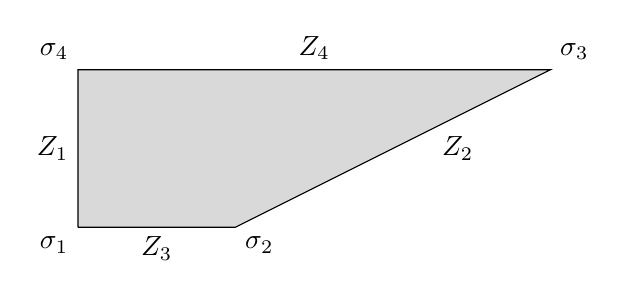
\begin{tikzpicture}
 \draw[fill=gray!30] (0,0)node[below left]{$\sigma_1$} --node[below]{$Z_3$} (2,0)node[below right]{$\sigma_2$} --node[right=.5cm]{$Z_2$} (6,2)node[above right]{$\sigma_3$} --node[above]{$Z_4$} (0,2)node[above left]{$\sigma_4$} --node[left]{$Z_1$} (0,0);
 \end{tikzpicture}
\end{center}
The cohomology ring is given by:
\[
 H^*(\mathbb F_2,\ZZ)\simeq\ZZ[Z_1,\ldots,Z_4]/\langle Z_1-Z_2,Z_4-Z_3-2Z_2, Z_1Z_2,Z_3Z_4\rangle
\]
We work out the following weights for the $\Gm^4$-action:

When thinking of them as curve classes, we'll write $F=[Z_1], D_0=[Z_4], D_\infty=[Z_3]$.

\begin{center}
 \begin{tabular}{||c|c||c|c||}
  \hline\hline
  $\lambda^{\sigma_1}_{\sigma_2}=-\lambda^{\sigma_2}_{\sigma_1}$ & $\lambda_1-\lambda_2$ & $\lambda^{\sigma_3}_{\sigma_4}=-\lambda^{\sigma_4}_{\sigma_3}$ & $\lambda_2-\lambda_1$ \\
  \hline
  $\lambda^{\sigma_2}_{\sigma_3}=-\lambda^{\sigma_3}_{\sigma_2}$ & $2\lambda_1+\lambda_3-\lambda_4$ & $\lambda^{\sigma_4}_{\sigma_1}=-\lambda^{\sigma_1}_{\sigma_4}$ & $\lambda_4-2\lambda_2-\lambda_3$ \\
  \hline\hline
 \end{tabular}
\end{center}

We are going to consider the space $\Q{0}{3}{\mathbb F_2}{D_\infty+F}$ (and the analogous stable maps space) with insertions $\xi_1=Z_3,\xi_2=Z_4,\xi_3=Z_1Z_4$.

The relevant graphs in the stable maps case are:
\begin{center}
 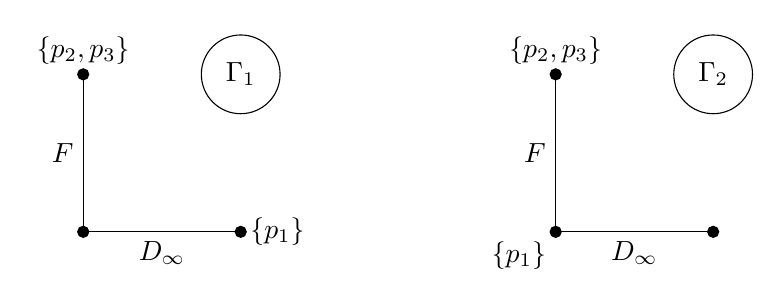
\begin{tikzpicture}[radius=2pt]
  \draw[fill=black] (0,2) circle node[above]{$\{p_2,p_3\}$};
  \draw[fill=black] (0,0) circle;
  \draw[fill=black] (2,0) circle node[right]{$\{p_1\}$};
  \draw (0,2) --node[left]{$F$} (0,0) -- node[below]{$D_\infty$} (2,0);
  \draw (2,2) circle (.5cm) node{$\Gamma_1$};
  %
  \draw[fill=black] (6,2) circle node[above]{$\{p_2,p_3\}$};
  \draw[fill=black] (6,0) circle node[below left]{$\{p_1\}$};
  \draw[fill=black] (8,0) circle;
  \draw (6,2) --node[left]{$F$} (6,0) -- node[below]{$D_\infty$} (8,0);
  \draw (8,2) circle (.5cm) node{$\Gamma_2$};
 \end{tikzpicture}
\end{center}
In the case of quasimaps $\Gamma_2$ is unstable instead the following graph must be taken into account:
\begin{center}
 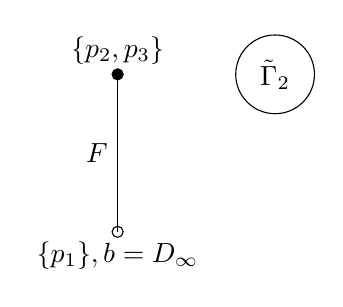
\begin{tikzpicture}[radius=2pt]
  \draw[fill=black] (0,2) circle node[above]{$\{p_2,p_3\}$};
  \draw[fill=white] (0,0) circle node[below]{$\{p_1\},b=D_\infty$};
  \draw (0,2) --node[left]{$F$} (0,0);
  \draw (2,2) circle (.5cm) node{$\tilde\Gamma_2$};
 \end{tikzpicture}
\end{center}
The white circle is supposed to indicate that there is a full basepoint component at that vertex.


\section{Relative quasimaps}
The relative problem in Gromov-Witten theory consists in studying maps with not only incidence, but also tangency conditions to a divisor. It has seen great advancements in the past twenty years, of which I will sample some most relevant ones in algebraic geometry (there is an almost parallel and similarly rich story in symplectic geometry):
\begin{itemize}
 \item R. Vakil's pioneering work on rational and elliptic curves in projective space, satisfying tangency conditions to a hyperplane \cite{Vre};
 \item A. Gathmnn's work in genus $0$, enhancing the previous one to the case of a smooth very ample divisor in any variety \cite{Ga};
 \item J. Li's moduli space of maps to expanded targets, removing the ampleness hypothesis on the divisor and developing the framework for the all important degeneration formula \cite{Li1,Li2}, which has been reviewed by B. Kim in a more explicitly logarithmic \cite{KimLog}, and by D. Abramovich and B. Fantechi in a more stacky \cite{AbramovichFantechi} context;
 \item a host of recent works around D. Abramovich, Q. Chen, M. Gross, and B. Siebert's space of logarithmic stable maps \cite{ChenLog,AbramovichChenLog,GrossSiebertLog}, which allows for example the divisor to be snc.
\end{itemize}
It would be interesting to have a full relative theory for $\epsilon$-quasimaps, including a degeneration formula and wall-crossing formulae for relative invariants as well; one application (suggested by I. Ciocan-Fontanine) would be to the study of the higher genus $\epsilon$-quasimap invariants of the quintic threefold via Maulik-Pandharipande's degeneration scheme \cite{MauPan}. In \cite{BN} we have made a first step towards this program, namely we have introduced spaces of genus $0$ relative quasimaps to a smooth very ample divisor, extending the work of Gathmann. Among the peculiarities of this approach are the fact that the tangency needs not be maximal (i.e. not all intersection points of the curve with the divisor must be marked with the respective tangency order requirement), and the fact that the relative spaces are nested (they become smaller as the tangency requirement gets higher), with a nice formula expressing their virtual classes in terms of one another, corrected by a boundary term exhibiting a clear recursive structure. This led Gathmann to the discovery of an algorithm for computing relative invariants, or, even further, restricted invariants of the hyperplane section, recursively, starting from the descendant theory of the ambient space; under positivity assumptions, he was able to realise this in a different proof of what goes under the name of Givental's mirror theorem, or the quantum Lefschetz principle \cite{Ga-MF}. In this section I will report on my work with N. Nabijou.
\subsection{Review of Gathmann's work} The starting point is the case of $\PP^N$ relative to a hyperplane $H$. The most down-to-earth approach works in this case: fixed a tangency condition $\alpha\in\N^n$ with $\sum\alpha\leq d$, Gathmann defines the relative space $\M{0}{\alpha}{\PP^N|H}{d}\subseteq \M{0}{n}{\PP^N}{d}$ as the closure of the ``nice'' locus of maps $f\colon(\PP^1,\mathbf x)\to \PP^N$ such that $f(\PP^1)\subsetneq H$ and $f^{-1}(H)-\sum\alpha_ix_i$ is an effective divisor. He then proves that the reducible maps that lie in the closure can be characterised combinatorially as follows:
 a stable map $(C,x_1, \ldots, x_n,f)$ is in $\M{0}{\alpha}{\PP^N|H}{d}$ if and only if, for each connected component $Z$ of $f^{-1}(H) \subseteq C$:
\begin{enumerate}
\item if $Z$ is a point and is equal to a marked point $x_i$, then $f$ is tangent to $H$ at $x_i$ to order at least $\alpha_i$;
\item if $Z$ is a curve, and if we let $C^{(i)}$ for $1 \leq i \leq r$ denote the irreducible components of $C$ adjacent to $Z$, and $m^{(i)}$ denote the multiplicity of $f|_{C^{(i)}}$ to $H$ at the node $Z \cap C^{(i)}$, then:
\begin{equation} \label{Relative stable map internal component inequality} H \cdot f_* [Z] + \sum_{i=1}^r m^{(i)} \geq \sum_{x_i \in Z} \alpha_i \end{equation}
\end{enumerate}
Now this definition works well for every pair $(X|Y)$ of a variety with a smooth divisor, by just replacing $H$ with $Y$ in the description above. On the other hand, the definition as the closure of the nice locus makes it clear that $\M{0}{\alpha}{\PP^N|}{d}$ is irreducible of the expected dimension: \[\dim(\M{0}{\alpha}{\PP^N|H}{d})=\dim (\M{0}{n}{\PP^N}{d})-\sum\alpha.\]
If we then assume that $Y$ is very ample, we may use the complete linear system assoiated to it in order to embed $\phi_{\lvert Y\rvert}\colon X\hookrightarrow\PP^N$ and find a hyperplane $H\subseteq \PP^N$ such that $H\cap X= Y$. Set $d=\phi_{\lvert Y\rvert,*}(\beta)$ for a curve class $\beta\in H_2^+(X)$. The following cartesian diagram holds true:
\bcd
\M{0}{\alpha}{X|Y}{\beta}\ar[d]\ar[r]\ar[dr,phantom,"\Box"] & \M{0}{n}{X}{\beta}\ar[d,"\Phi_{\lvert Y\rvert}"] \\
\M{0}{\alpha}{\PP^N|H}{d} \ar[r] & \M{0}{n}{\PP^N}{d}
\ecd
Furthermore $\operatorname{R}^\bullet\pi_*f^*N_{X/\PP^N}$ provides a perfect obstruction theory for $\Phi_{\lvert Y\rvert}$, hence we may endow $\M{0}{\alpha}{X|Y}{\beta}$ with a virtual class
\[ \virt{\M{0}{\alpha}{X|Y}{\beta}}=\Phi_{\lvert Y\rvert}^![\M{0}{\alpha}{\PP^N|H}{d}] \]
which also has the expected codimension $\sum\alpha$ with respect to $\virt{\M{0}{n}{X}{\beta}}$.

As anticipated, the combinatorial description shows that $\M{0}{\alpha+e_k}{X|Y}{\beta}\subseteq \M{0}{\alpha}{X|Y}{\beta}$, and it is a divisor. Gathmann finds a natural line bundle with section that cuts it out, together with a number of boundary correction terms. Let me start with some heuristics: assume $n=1$ for this. Let $Y=V(s)\subseteq X$. Then $\M{0}{(1)}{X|Y}{\beta}\subseteq \M{0}{1}{X}{\beta}$ is cut out by the section $\ev_1*(s)$ of $\ev_1^*\OO_X(Y)$. Now the restriction of $\ev_1$ to $\M{0}{(1)}{X|Y}{\beta}$ maps to $Y$; by composing $df_{x_1}\colon TC_{x_1}\to TX_{f(x_1)}$ with the projection to $N_{Y/X,x_1}$ we get a map that has to vanish if $f$ is tangent to $H$ at $x_1$. Rearranging we get a section $\ev_1^*(d^1s)$ of $x_1^*(T^*C)\otimes\ev_1^*\OO_X(Y)$ that defines $\M{0}{(2)}{X|Y}{\beta}$ within $\M{0}{(1)}{X|Y}{\beta}$. More generally we may use the jet bundles (or bundles of principal parts) of $\OO_X(Y)$: there is an exact sequence
\[ 0\to x_1^*\Omega_{C}^{\otimes m+1}\otimes\ev_1^*\OO_X(Y)\to ev_1^*\mathcal P^{m+1}(\OO_X(Y))\to ev_1^*\mathcal P^{m}(\OO_X(Y))\to 0\]
and $s$ induces a section $\ev_1^*(d^{m+1}s)$ of the middle term (which should be thought of as the Taylor expansion up to order $m+1$ of $s$ at $x_1$), the image of which in the rightmost term (i.e. its truncation up to order $m$) vanishes on $\M{0}{(m)}{X|Y}{\beta}$, hence inducing a section of the line bundle $x_1^*\Omega_{C}^{\otimes m+1}\otimes\ev_1^*\OO_X(Y)$ which vanishes along $\M{0}{(m+1)}{X|Y}{\beta}$. Notice though that it also vanishes (for every $m$, really) on those maps such that the irreducible component containing $x_1$ lies entirely inside $Y$. We have thus arrived to Gathmann's formula:
\begin{thm}\cite[Theorem 2.6]{Ga}\label{thm:Gathmann_formula} In the Chow group of $\M{0}{\alpha}{X|Y}{\beta}$
 \begin{equation*} (\alpha_k \psi_k + \ev_k^* \OO_X(Y)) \cap \virt{\M{0}{\alpha}{X|Y}{\beta}} = \virt{\M{0}{\alpha+e_k}{X|Y}{\beta}} + \virt{\mathcal{D}_{\alpha,k}(X,\beta)} \end{equation*}
\end{thm}
where $\mathcal{D}_{\alpha,k}(X,\beta)$ is a sum over all $r\geq 0$ determining the number of adjacent external components $C^{(1)},\ldots,C^{(r)}$, $M=(m^{(1)},\ldots,m^{(r)})\in \N^r_{>0}$ determining the order of contact of $C^{(i)}$ with $Y$ at the intersection with the internal component $C^{(0)}$, $A=(\alpha^{(0)},\ldots,\alpha^{(r)})$ and $B=(\beta_0,\ldots,\beta_r)$ dictating the splitting of the markings/tangency requirements and curve class respectively, of the following ``comb loci'':
\[\mathcal{D}_{A,B,M}(X)=\M{0}{\lvert\alpha^{(0)}\rvert+r}{Y}{\beta_0}\times_{H^r}\prod_{i=1}^r
\M{0}{\alpha^{(i)}\cup m^{(i)}}{X|Y}{\beta_i}\]
These are endowed with the product virtual fundamental class, weighted by a factor $\frac{m^{(1)}\cdot\ldots\cdot m^{(r)}}{r!}$; the denominator is just there to make the extra gluing markings unordered, while in a sense the numerator is the real content of Gathmann's formula. As noticed above the section $\ev_k^*(d^ms)$ vanishes whenever $x_k$ lies on an internal component; the sum must therefore run over all those splitting types such that $\mathcal{D}_{A,B,M}(X)$ lies in $\M{0}{\alpha}{X|Y}{\beta}$ but not in $\M{0}{\alpha+e_k}{X|Y}{\beta}$, namely those satisfying $\alpha_k\in\alpha^{(0)}$ and
\[\OO_X(Y)\cdot\beta_0+\sum M=\sum \alpha^{(0)}.\]
The proof goes roughly as follows: the reduction to the case of $(\PP^N|H)$ is just a matter of virtual intersection calculus; in the unobstructed case the shape of the formula follows simply from the above arguments and a(n actual) dimension computation, so the hard part is to get the coefficients right. Locally one may reduce further to $(\PP^1,\{\infty\})$ by projecting from a generic $(N-2)$-plane inside $H$; finally the proof for $\PP^1$ is based on Vakil's observation that, for maps from cuves to curves, the obstruction theory only sees the special loci (markings, nodes, ramification points, and contracted components), so that one can split the deformation space and reduce to a much simpler moduli problem.
\begin{rmk}
 Gathmann's recursion can be recovered in the framework of Jun Li's spaces of maps to expansions (or rather Kim's logarithmic stable maps) when the target is $(\PP^N|H)$. This was suggested by J. Wise and D. Ranganathan. It is in a sense surprising because one gets the non-maximal from the maximal tangency case; but in fact this idea was already contained in the proof of Gathmann's formula. Here is how we can recover Theorem \ref{thm:Gathmann_formula}: add $h=d-\sum\alpha$ auxiliary markings of multiplicity $1$, so consider $\MK{0}{\alpha\cup(1,\ldots,1)}{\PP^N|H}{d}$; forgetting the auxiliary markings and the log structures, collapsing the target, and stabilising the source curve, we get an $(h!:1)$ cover of $\M{0}{\alpha}{\PP^N|H}{d}$ (generically we are just marking the $h$ simple intersections of the image of $C$ with $H$, and endowing $C$ with the pullback of the divisorial log structure on $\PP^N$; here we use that $g=0$ and the target is $\PP^N$, but notice that the approach will work whenever the nice locus is dense in the relative space). Denote by $c\colon \MK{0}{\alpha\cup(1,\ldots,1)}{\PP^N|H}{d}\to \M{0}{\alpha\cup(1,\ldots,1)}{\PP^N}{d}$ the map that forgets the log structures, collapses the target, and stabilises the source curve; we may then pullback Gathmann's line bundle and section along $c$. The vanishing locus of the section thus obtained consists of maps such that the target is expanded, and $x_k$ lies on a non-trivial (i.e. having either positive horizontal degree, or at least three markings) component at higher level. Notice that, as soon as there is more than one non-trivial component at higher level, collapsing the target has positive-dimensional fibers. Hence we are reduced to a sum over bipartite graphs with only one vertex at higher level; we recognise in these the shape of the comb loci appearing in Gathmann's formula. Also, I claim that the only case in which one of the auxiliary markings (say $x_{n+1}$) may lie on the component containing $x_k$ is when the latter only contains $x_k$ and $x_{n+1}$ among the markings, and has zero horizontal degree  - otherwise the map collapsing the target and forgetting the auxiliary markings will have positive dimensional fibers. The first case recovers exactly $\M{0}{\alpha+e_k}{\PP^N|H}{d}$! The claim follows from the fact that the rubber space $\M{0}{\alpha}{\PP_H(\OO\oplus\OO(1))}{\beta}\tilde{}\ $ has the same dimension as $\M{0}{\lvert\alpha\rvert}{H}{\beta}$, see \cite[\S 2.4]{GraberVakil}. Now the coefficient with which each of these loci appears has been computed by several authors in the framework of the degeneration formula (see e.g. \cite[Remark 6.3.1.2]{KimLog} and \cite[Equation (1.7)]{KLR}):  the log structure is determined at the level of ghost sheaves by the underlying morphism, and the numerator counts the number of log liftings, \marginnote{CHECK ME} while the denominator again clears out the ordering of the edges. There is already in Gathmann's proof a subtelty, that $\M{0}{\alpha+e_k}{\PP^N|H}{d}$ on one side comes with a coefficient $\alpha_k+1$, while on the other side it comes with an $\alpha_k$ from the comparison between $\psi_k$ and $\fgt_{n+1,\ldots,n+h}^*\psi_k$. All the degeneracy loci that persist under pushforward cover $(h!:1)$ one of the comb loci in Gathmann's formula.
\end{rmk}

\subsection{Definitions and propositions}
I come now to the definition of relative quasimaps \cite[\S 2.3]{BN}. Let $X$ be a smooth toric variety, $Y=V(s)$ a smooth very ample divisor (not necessarily toric). As in the discussion of functoriality above, we may write $\OO_X(Y)=\bigotimes_{\rho\in\Sigma(1)}\OO_X(D_\rho)^{\otimes a_\rho}$ and 
\[s=\sum_{\mathbf a:[\mathbf a]=\OO_X(Y)}\mu_{\mathbf a}\prod_{\rho\in\Sigma(1)}z_\rho^{a_\rho}\]
in terms of Cox's homogeneous coordinates. For a quasimap 
\[ \Big((C,x_1,\ldots,x_n), (L_\rho,u_\rho)_{\rho \in \Sigma(1)}, (\varphi_m)_{m \in M}\Big) \]
set $L_Y=\bigotimes_{\rho\in\Sigma(1)}L_\rho^{\otimes a_\rho}$ and
\[u_Y=\mu_{\mathbf a}\prod_{\rho\in\Sigma(1)}u_\rho^{a_\rho}+\sum_{\mathbf a\neq \mathbf b:[\mathbf b]=\OO_X(Y)}\mu_{\mathbf b}\varphi_{\mathbf b-\mathbf a}\left(\prod_{\rho\in\Sigma(1)}u_\rho^{b_\rho}\right).\]
%\appendix
\begin{definition}
 A quasimap belongs to the relative space $\Q{0}{\alpha}{X|Y}{\beta}\subseteq \Q{0}{n}{X}{\beta}$ if for every connected component $Z$ of $s_Y^{-1}(0)$, the following holds:
\begin{enumerate}
\item if $Z$ is a point and is equal to a marked point $x_i$, then $s_Y^*(0)$ has order at least $\alpha_i$ at $x_i$;
\item if $Z$ is a curve, and if we let $C^{(i)}$ for $1 \leq i \leq r$ denote the irreducible components of $C$ adjacent to $Z$, and $m^{(i)}$ denote the multiplicity of $f|_{C^{(i)}}$ to $H$ at the node $Z \cap C^{(i)}$, then:
\begin{equation} \label{Relative quasimap internal component inequality} \deg(L_{Y}|_Z) + \sum_{i=1}^r m^{(i)} \geq \sum_{x_i \in Z} \alpha_i \end{equation}
\end{enumerate}
\end{definition}

I am going to discuss an adaptation of Gathmann's recursion formula to this setup: the idea is simply to push down Theorem \ref{thm:Gathmann_formula} along the collapsing morphism in the case of $(\PP^N|H)$, and then recover the general formula by virtual pullback.

\begin{lem}
 The collapsing morphism $\chi$ restricts to a proper and birational morphism \[\chi_\alpha\colon \M{0}{\alpha}{\PP^N|H}{d}\to \Q{0}{\alpha}{\PP^N|H}{d}.\]
\end{lem}
\begin{proof}
 Fix coordinates on $\PP^N$ such that $H=\{x_0=0\}$. We first show that a stable map satisfying \eqref{Relative stable map internal component inequality} is sent to a quasimap satisfying \eqref{Relative quasimap internal component inequality}: the collapsing of rational tails happens far from any markings, so we only have to discuss the case of an internal component $Z$. If the rational tail $R$ is internal, then collapsing does not affect the left hand side of the inequality (it simply transfers some degree from $R$ to $\overline{Z\setminus R}$); on the other hand, if it is external, collapsing may only increase the left hand side, since the multiplicity of contact $m^R$ is at most equal to the degree of $f_{|R}$. This proves that $\chi(\M{0}{\alpha}{\PP^N|H}{d})\subseteq \Q{0}{\alpha}{\PP^N|H}{d}$.
 
 On the other hand $\chi_\alpha$ is surjective: given a relative quasimap $\xi'$ with an internal basepoint $q_0$ of order $d_0$, choose any line $\ell$ through its image, with $\ell$ transverse to $H$, and lift $\xi'$ to a stable map $\xi$ by adjoining a $\PP^1=:R$ to the source curve at $q_0$, and defining the map $f_{|R}$ to be a $d_0$-fold cover of $\ell$ totally ramified at $q_0$ (any basepoint which is not internal is easier to deal with). Now, given any relative quasimap $\xi'\in\Q{0}{\alpha}{\PP^N|H}{d}$ we may choose a lifting $\xi\in\M{0}{\alpha}{\PP^N|H}{d}$; by Gathmann's result, $\xi$ can be smoothed to a map in the nice locus; applying $\chi$ to such a smoothing we obtain a smoothing of $\xi'$. This shows that $\Q{0}{\alpha}{\PP^N|H}{d}$ is contained in the closure of the nice locus of relative quasimaps with no basepoints and image not contained in $H$. On the other hand $\Q{0}{\alpha}{\PP^N|H}{d}$ is closed by the conservation of number principle. Therefore $\chi_\alpha$ is proper and birational, being an isomorphism on the nice locus.
\end{proof}

\begin{prop}\label{prop:quasimap_Gathmann_formula} In the Chow group of $\Q{0}{\alpha}{X|Y}{\beta}$
 \begin{equation*} (\alpha_k \psi_k + x_k^*c_1(L_Y)) \cap \virt{\Q{0}{\alpha}{X|Y}{\beta}} = \virt{\Q{0}{\alpha+e_k}{X|Y}{\beta}} + \virt{\mathcal{D}^Q_{\alpha,k}(X,\beta)} \end{equation*}
\end{prop}
Notice that $\mathcal{D}^Q_{\alpha,k}(X,\beta)$ is a sum of ``comb loci'', running over all splittings $A,B,M$ of the markings, curve class, and multiplicities at the internal-to-external nodes, this time required to satisfy the quasimap stability condition, namely there are no rational tails:
\[\mathcal{D}^Q_{A,B,M}(X)=\Q{0}{\lvert\alpha^{(0)}\rvert+r}{Y}{\beta_0}\times_{H^r}\prod_{i=1}^r
\Q{0}{\alpha^{(i)}\cup m^{(i)}}{X|Y}{\beta_i}\]
endowed with the product virtual fundamental class, weighted by a factor $\frac{m^{(1)}\cdot\ldots\cdot m^{(r)}}{r!}$.
\begin{proof}
 In the case of $(\PP^N|H)$ the formula follows by pushing forward Gathmann's formula along $\chi$: for this it is useful to notice that
 \begin{equation}
  \chi^*(\psi_k)=\psi_k, \quad \text{and} \quad \chi^*(x_k^*L_Y)=\ev_k^*\OO_X(Y),
 \end{equation}
because collapsing does not affect the universal curve in a neighbourhood of the marking $x_k$. On the other hand if a comb locus $\mathcal{D}^Q_{A,B,M}(X)$ contains a rational tail (necessarily external), then the restriction of $\chi$ to $\mathcal{D}^Q_{A,B,M}(X)$ has positive dimensional fibers, because $\dim(\M{0}{(m^{(i)})}{\PP^N|H}{d})>\dim H$, so the corresponding term of Gathmann's formula vanishes under $\chi_*$.

The case of a smooth very ample divisor $(X|Y)$ follows by virtual pullback: $\Q{0}{n}{\PP^N}{d}$ is unobstructed, hence the  closed embedding $\phi_{\lvert Y\rvert}\colon X\hookrightarrow \PP^N$ induces $\Phi_{\lvert Y\rvert}\colon \Q{0}{n}{X}{\beta}\to \Q{0}{n}{\PP^N}{d}$ endowed with a perfect obstruction theory. $\Phi_{\lvert Y\rvert}^!\virt{\Q{0}{\alpha}{\PP^N|H}{d}}=\virt{\Q{0}{\alpha}{X|Y}{\beta}}$ by the very definition of the latter, and it is easily checked that $\Phi_{\lvert Y\rvert}^!\virt{\Q{0}{a_0+r}{H}{d_0}}=\virt{\Q{0}{a_0+r}{Y}{\beta_0}}$ where the latter is defined as in \cite{CFKM}. The claim follows from a careful application of the splitting property of the virtual class of quasimap spaces; the details are checked in \cite[\S 4 and Appendix B.4]{BN}.
\end{proof}

\subsection{Gathmann's algorithm and quasimap quantum Lefschetz} Notice that in the very last step of the recursion, i.e. increasing $\sum\alpha$ from $Y\cdot \beta$ to $Y\cdot \beta+1$, there is no main term but only boundary corrections; also, one of them represent maps with no external components, which recovers $\Q{0}{n}{Y}{\beta}$.

Gathmann describes an algorithm for computing relative invariants of $(X|Y)$ and \ilemph{restricted} absolute invariants of $Y$ (i.e. the cohomological insertions all lie in the image of the restriction map $H^*(X)\to H^*(Y)$) recursively, assuming that we know the descendant invariants of $X$. The proof is by induction on $d=Y\cdot \beta, n,$ and $\sum\alpha$ (where we set $\sum\alpha=d+1$ when looking at absolute invariants of $Y$). If we want to compute a relative invariant with tangency condition $\alpha$ and degree $\beta$, assume $\alpha_k>0$ (if we cannot find such a $k$ then we are just considering an absolute invariant of $X$); we may then write down the formula as
\[\virt{\Q{0}{\alpha}{X}{\beta}}=((\alpha_k-1)\psi_k+\ev_k^*\OO_X(Y))\virt{\Q{0}{\alpha-e_k}{X}{\beta}}-\virt{\mathcal{D}^Q_{\alpha-e_k,k}(X,\beta)}.\]
The classes appearing on the right hand side have lower numerical invariants, so we may assume they have been computed inductively. There is one subtlety, namely that we use the cohomological splitting of the diagonal of $Y\times Y$ in order to reduce the integral on the right hand side to a product of relative $(X|Y)$ and absolute $Y$ invariants, but in doing so we might introduce some non-restricted insertions. It can be proved that invariants of $Y$ comprising only one unrestricted insertion vanish: assume we are interested in $\langle\tau_{a_1}(\delta_1),\ldots,\tau_{a_n}(\delta_n)\rangle^{\epsilon,Y}_{0,n\beta}$ with only $\delta_1\in i^*H^*(X)^\perp$. Then recall that $i_*\virt{\Q{0}{n}{Y}{\beta}}=c_{top}(\pi_*f^*\OO_X(Y))\cap \virt{\Q{0}{n}{X}{i_*\beta}}$, and we may write $c_{top}(\pi_*f^*\OO_X(Y))=\ev_1^*\OO_X(Y)c_{top}(E^{Y\cdot\beta})$. We may factor through the following diagram:
\bcd
\Q{0}{(1,0,\ldots,0)}{X|Y}{\beta}\ar[r,"j"]\ar[d,"\tilde\ev_1"] & \Q{0}{n}{X}{\beta}\ar[d,"\ev_1"] \\
Y\ar[r,"i"] & X
\ecd
and $\langle\tau_{a_1}(\delta_1),\ldots,\tau_{a_n}(\delta_n)\rangle^{\epsilon,Y}_{0,n\beta}$ is computed by
\begin{multline*}
 \delta_1\cdot\tilde\ev_{1,*}i^!\left(\psi_1^{a_1}\prod_{i=2}^n\ev_i^*(\delta_i)\psi_i^{a_i}c_{top}(E^{Y\cdot\beta})\cap\virt{\Q{0}{n}{X}{\beta}}\right)= \\
 \delta_1\cdot i^*\ev_{1,*}\left(\psi_1^{a_1}\prod_{i=2}^n\ev_i^*(\delta_i)\psi_i^{a_i}c_{top}(E^{Y\cdot\beta})\cap\virt{\Q{0}{n}{X}{\beta}}\right) =0
\end{multline*}
It is possible then to prove recursively that any relative invariant with only one unrestricted invariant vanishes, and this is sufficient for our application, since the external components always get at most one such insertion.

\smallskip

The above algorithm can be realised into a compact formula relating some quasimap invariants of $Y$ to those of $X$ under some positivity assumption, which allows us to discard most contributions from the comb loci by dimensional reasons. The following discussion is inspired by \cite{Ga-MF}, in which Gathmann applies the stable map recursion formula to obtain a new proof of the mirror theorem for hypersurfaces \cite{Givental-equivariantGW}.

From now on we make the following two assumptions:
\begin{enumerate}
\item \emph{$Y$ is semi-positive}: $-K_Y$ is nef;
\item \emph{$Y$ contains all curve classes}: the map $i_* : \Achow_1(Y) \to \Achow_1(X)$ is surjective.
\end{enumerate}
\begin{rmk}
 By adjunction, $-K_X$ pairs strictly positively with every curve class coming from $Y$, hence with every curve class by Assumption (2). Thus $-K_X$ is ample, or in other words, $X$ is Fano, by Kleiman's criterion, since the effective cone of the toric variety $X$ is finitely generated in $\Achow_1(X)$, hence is closed in $\Achow_1(X)_{\mathbb{R}}$. Also note that if $\dim X \geq 3$ then Assumption (2) always holds, due to the classical Lefschetz hyperplane theorem; on the other hand if $\dim X = 2$ then Assumption (2) forces $X$ to be $\PP^2$.
\end{rmk}

We fix a homogeneous basis $\eta_0, \ldots, \eta_k$ for $\HH^*(X) = \HH^*(X,\QQ)$ and let $\eta^0, \ldots, \eta^k$ denote the dual basis with respect to the Poincar\'e pairing. Without loss of generality we may suppose that $\eta^0=\mathbbm 1_X$ and $\eta^1=[Y]$. We get an induced basis $\rho_1=i^*\eta_1, \ldots, \rho_k = i^* \eta_k$ for $i^*\HH^*(X)$. Notice that $\rho_0 = i^* \eta_0 = i^* [\pt_X] = 0$, $\rho_1 = i^* \eta_1 = [\pt_Y]$.  We can extend the $\rho_i$ to a basis $\rho_1, \ldots, \rho_l$ for $\HH^*(Y)$ by adding $\rho_{k+1}\ldots,\rho_{l}$. Let $\rho^1, \ldots, \rho^l$ denote the dual basis; notice that $\rho^i$ is \emph{not} equal to $i^* \eta^i$ (they do not even have the same degree!).  Note also that $\rho^1 = \mathbbm{1}_Y$.

We are going to analyse the behaviour of a generating function of $2$-pointed quasimap invariants with a fundamental class insertion, which in fact coincides with the small $I$-function from Section \ref{subsec:gf_and_wc}. Let me fix some more notation for this section.

For any smooth projective toric variety\footnote{Or more generally any space for which the quasimap invariants are defined, for instance a smooth hypersurface in a toric variety.} $X$ and any effective curve class $\beta\in \HH_2^+(X)$, we define
\begin{align*} S_0^X(z,\beta) & =(\ev_1)_*\left(\frac{1}{z-\psi_1} \virt{\Q{0}{2}{X}{\beta}}\right) 
\intertext{and}
S_0^X(z,q) &=\sum_{\beta\geq 0} q^\beta S_0^X(z,\beta)\end{align*}
where by convention $S_0^X(z,0)= \mathbbm 1_X$, and $q$ is a Novikov variable. These are generating functions for quasimap invariants of $X$ which take values in $\HH^*(X)$.

The same definition applies to $Y$. However, sometimes we may wish to consider only insertions of cohomology classes coming from $X$. These are the so-called \emph{restricted quasimap invariants}, and the corresponding generating function is defined as
\begin{equation*} \tilde{S}^Y_0(z,\beta) = (\ev_1)_* \left( \dfrac{1}{z-\psi_1} \virt{\Q{0}{2}{Y}{\beta}} \right) \end{equation*}
where crucially $\ev_1$ is viewed as \emph{mapping to $X$} instead of to $Y$. Thus $\tilde{S}^Y_0(z,\beta)$ takes values in $\HH^*(X)$ and involves only quasimap invariants of $Y$ with insertions coming from $i^*\HH^*(X)$; this is in contrast to $S^Y_0(z,\beta)$, which takes values in $\HH^*(Y)$ and involves quasimap invariants of $Y$ with arbitrary insertions. As earlier, we can also define $\tilde{S}_0^Y(z,q)$.

Now, since $X$ and $Y$ are smooth, we may use Poincar\'{e} duality to define a push-forward map on cohomology, $i_* \colon \HH^k(Y) \to \HH^{k+2}(X)$.

\begin{lemma} $i_* S^Y_0(z,\beta) = \tilde{S}^Y_0(z,\beta)$. \end{lemma}
\begin{proof} This follows from functoriality of cohomological push-forwards and the fact that we have a commuting triangle:
\bcd
\Q{0}{2}{Y}{\beta} \ar[rr,"\ev_1"] \ar[rd,"\ev_1" left=0.2cm] & & Y \ar[ld,"i"] \\
& X & 
\ecd
Let us spell this out explicitly, in order to help familiarise the reader with the generating functions involved. First, it is easy to see from the projection formula that:
\begin{align*} i_* \rho^i =
\begin{cases} \eta^i \qquad \text{for $i = 1, \ldots, k$} \\
0 \qquad \text{\ for $i = k+1, \ldots, l$} \end{cases} \end{align*}
Now, we can write $S_0^Y(z,\beta)$ as:
\begin{equation*} S_0^Y(z,\beta) = \sum_{i=1}^l \left\langle \dfrac{\rho_i}{z-\psi_1} , \mathbbm{1}_Y \right\rangle_{0,2,\beta}^Y  \rho^i \end{equation*}
Thus applying $i_*$ gives
\begin{align*} i_* S_0^Y(z,\beta)  = \sum_{i=1}^l \left\langle \dfrac{\rho_i}{z-\psi_1} , \mathbbm{1}_Y \right\rangle_{0,2,\beta}^Y   i_* \rho^i
= \sum_{i=1}^k \left\langle \dfrac{\eta_i}{z-\psi_1}, \mathbbm{1}_X \right\rangle_{0,2,\beta}^Y   \eta^i = \tilde{S}_0^Y(z,\beta) \end{align*}
as claimed. \end{proof}

\subsection{Quasimap Lefschetz formula} We now turn to our main result: a formula expressing the generating function $\tilde{S}_0^Y(z,q)$ for restricted quasimap invariants of $Y$ in terms of the quasimap invariants of $X$.

\begin{thm} \label{Theorem Quantum Lefschetz}
Let $X$ and $Y$ be as above. Then
\begin{equation}\label{eqn:mirror}
\dfrac{\sum_{\beta\geq 0} q^\beta\prod_{j=0}^{Y\cdot\beta}(Y+jz)S_0^X(z,\beta)}{P_0^X(q)}= \tilde{S}_0^Y(z,q)
\end{equation}
where:
\begin{align*}
 P_0^X(q) % & = 1 + \sum_{\substack{\beta>0 \\ K_Y\cdot\beta=0}} q^\beta (Y\cdot\beta) \langle [\pt_Y],\mathbbm 1_{X}\rangle_{0,(Y\cdot\beta,0),\beta}^{X|Y} \\
            & = 1 + \sum_{\substack{\beta>0 \\ K_Y\cdot\beta=0}} q^\beta(Y\cdot\beta)!\langle [\pt_X] \psi_1^{Y\cdot\beta-1} ,\mathbbm 1_{X}\rangle_{0,2,\beta}^X
\end{align*}
Notice that $P_0^X(q)$ depends not only on $X$ but also on the divisor class of $Y$ in~$X$; the superscript is supposed to indicate that the definition only involves quasimap invariants of $X$.
\end{thm}

\begin{proof}
For $m = 0, \ldots, Y \cdot \beta$, define the following generating function for $2$-pointed relative quasimap invariants
 \[
  S_{0,(m)}^{X|Y}(z,\beta)=(\ev_1)_*\left(\frac{1}{z-\psi_1}\virt{\Q{0}{(m,0)}{X|Y}{\beta}}\right)
 \]
where we view $\ev_1$ as mapping to $X$.  Note that  $S_{0,(0)}^{X|Y}(z,\beta) = S_0^X(z, \beta)$. Also define the following generating function for ``comb loci invariants''
\[
 T_{0,(m)}^{X|Y}(z,\beta)=(\ev_1)_*\left(m \virt{\Q{0}{(m,0)}{X|Y}{\beta}}+\frac{1}{z-\psi_1} \virt{\mathcal{D}^{\mathcal{Q}}_{(m,0),1}(X|Y,\beta)} \right)
\]
where again we view $\ev_1$ as mapping to $X$. As in \cite[Lemma 1.2]{Ga-MF}, it follows from Theorem \ref{Theorem general recursion} that
\begin{equation}
 (Y+mz) S_{0,(m)}^{X|Y}(z,\beta) = S_{0,(m+1)}^{X|Y}(z,\beta)+ T_{0,(m)}^{X|Y}(z,\beta)
\end{equation}
and we can apply this repeatedly to obtain:
\begin{equation} \label{eqn:G}
\prod_{j=0}^{Y\cdot\beta}(Y+jz) S_0^X(z,\beta) = \sum_{m=0}^{Y\cdot\beta}\prod_{j=m+1}^{Y\cdot\beta}(Y+jz)T_{0,(m)}^{X|Y}(z,\beta)
\end{equation}
We now examine the right-hand side in detail. By definition, $T_{0,(m)}^{X|Y}(z,\beta)$ splits into two parts: those terms coming from the relative space and those terms coming from the comb loci.

Let us first consider the contribution of the comb loci. Since there are only two marked points and the first is required to lie on the internal component of the comb, it follows from the strong stability condition that there are only two options: a comb with zero teeth or a comb with one tooth.

First consider the case of a comb with zero teeth. The moduli space is then $\Q{0}{2}{Y}{\beta}$ and we require that $Y \cdot \beta = m$. Thus this piece only contributes to $T_{0,(Y\cdot\beta)}^{X|Y}(z,\beta)$, and the contribution is:
\begin{equation*} \sum_{i=1}^k \left\langle \dfrac{\rho_i}{z-\psi_1}, \mathbbm{1}_Y \right\rangle_{0,2,\beta}^Y \eta^i \end{equation*}

Next consider the case of a comb with one tooth. Let $\beta^{(0)}$ and $\beta^{(1)}$ denote the curve classes of the internal and external components, respectively, and let $m^{(1)}$ be the contact order of the external component with $Y$. The picture is as follows
\begin{center}
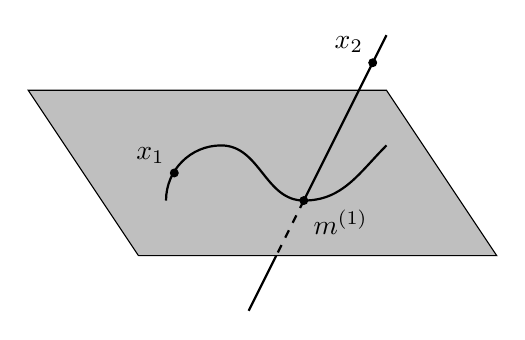
\begin{tikzpicture}[scale=0.7]
  \draw [fill=gray!50] (-.5,-1) -- (6,-1) -- (4,2) -- (-2.5,2) -- (-.5,-1);
  \draw [thick] (0,0) to [out=90,in=180] (1,1) to [out=0,in=180] (2.5,0) to [out=0,in=-135] (4,1);
  \draw [thick] (2.5,0) to (4,3);
  \draw [thick,dashed] (2.5,0) to (2,-1);
  \draw [thick] (2,-1) -- (1.5,-2);
  \draw [fill] (3.75,2.5) circle [radius=2pt] node[above left]{$x_2$};
  \draw [fill] (.15,.5) circle [radius=2pt] node[above left]{$x_1$};
  \draw [fill] (2.5,0.0) circle [radius=2pt] node[below right]{$m^{(1)}$};
 \end{tikzpicture}
\end{center}
and the invariants which contribute take the form
\begin{equation*} \bigg\langle \dfrac{\rho_i}{z-\psi_1},\rho^h\bigg\rangle_{0,2,\beta^{(0)}}^Y \bigg\langle \rho_h, \mathbbm 1_{X}\bigg\rangle_{0,(m^{(1)},0),\beta^{(1)}}^{X|Y} \end{equation*}
for $i = 1, \ldots, k$ and $h = 1, \ldots, l$. By computing dimensions, we find
\begin{align*}
0\leq \codim \rho^h &= \dim Y-\codim \rho_h \\
&= \dim Y-\vdim \Q{0}{(m^{(1)},0)}{X|Y}{\beta^{(1)}} \\
&= \dim Y-(\dim X-3-K_{X}\cdot \beta^{(1)}+2-m^{(1)})\\
&= K_Y \cdot \beta^{(1)} - Y \cdot \beta^{(1)}+m^{(1)} \\
&\leq 0
\end{align*}
where the final equality follows from adjunction and the final inequality holds because $-K_Y$ is nef and $m^{(1)}\leq Y \cdot \beta_1$. This shows that the only non-trivial contributions come from curve classes $\beta^{(1)}$ such that $K_Y \cdot \beta^{(1)}=0$, and that in this case the order of tangency must be maximal, i.e. $m^{(1)}=Y \cdot \beta^{(1)}$. Furthermore we must have $\codim \rho^h = 0$ and so $\rho^h = \rho^1 = \mathbbm{1}_Y$ which implies $\rho_h = \rho_1 = [\pt_Y]$. Finally since $m^{(1)}=Y \cdot \beta^{(1)}$ we have
\begin{equation*} m = Y \cdot \beta^{(0)}+m^{(1)}=Y \cdot (\beta^{(0)} + \beta^{(1)}) = Y \cdot \beta \end{equation*}
and so again this piece only contributes to $T_{0,(Y\cdot\beta)}^{X|Y}(z,\beta)$, and the contribution is:
\begin{equation*} \sum_{i=1}^k \left( \sum_{\substack{0 < \beta^{(1)} < \beta \\ K_Y \cdot \beta^{(1)}=0}} (Y \cdot \beta^{(1)}) \bigg\langle \dfrac{\rho_i}{z-\psi_1}, \mathbbm{1}_Y \bigg\rangle_{0,2,\beta-\beta^{(1)}}^Y \bigg\langle \rho_1, \mathbbm{1}_X \bigg\rangle_{0,(Y \cdot \beta^{(1)},0),\beta^{(1)}}^{X|Y} \right) \eta^i \end{equation*}
where the $Y \cdot \beta^{(1)}$ factor comes from the weighting on the virtual class of the comb locus. Finally, we must examine the terms of $T_{0,(m)}^{X|Y}(z,\beta)$ coming from:
\begin{equation*}\ev_{1*}(m\virt{\Q{0}{(m,0)}{X|Y}{\beta}})\end{equation*} 
Notice that we only have insertions from $i^*\HH^*(X) \subseteq \HH^*(Y)$, since $\ev_1$ is viewed as mapping to $X$. On the other hand
\begin{align*} \vdim \Q{0}{(m,0)}{X|Y}{\beta} & = \dim X-3 -K_X \cdot \beta +2-m & \\
& = \dim X - 1 -K_Y \cdot \beta + Y \cdot \beta - m \ \ & \text{by adjunction} \\
& \geq \dim X - 1 + Y\cdot\beta - m \ \ & \text{since $-K_Y$ is nef} \\
& \geq \dim X - 1 \ \ & \text{since $m \leq Y \cdot \beta$} \end{align*}
where in the second line we have applied the projection formula to $i$, and thus have implicitly used Assumption (2), discussed in \S \ref{Subsection setup}; namely that every curve class on $X$ comes from a class on $Y$.

Consequently the only insertions that can appear are those of dimension $0$ and $1$. However, the restriction of the $0$-dimensional class $\eta_0 = [\pt_X]$ to $Y$ vanishes, as do the restrictions of all $1$-dimensional classes except for $\eta_1$ (by the definition of the dual basis, since $\eta^1 = Y$). Thus the only insertion is $i^*\eta_1=\rho_1=[\pt_Y]$, and since $\eta^1$ has dimension $1$ all the inequalities above must actually be equalities. Thus we only have a contribution if $-K_Y \cdot \beta = 0$ and $m = Y \cdot \beta$. The contribution to $T_{0,(Y\cdot\beta)}^{X|Y}(z,\beta)$ in this case is:
\begin{equation*} (Y \cdot \beta) \langle \rho_1 , \mathbbm{1}_X \rangle_{0,(Y \cdot \beta,0),\beta}^{X|Y} \eta^1 \end{equation*}

Thus we have calculated $T_{0,(m)}^{X|Y}(z,\beta)$ for all $m$; substituting into equation \eqref{eqn:G} we obtain
\begin{align*} \prod_{j=0}^{Y \cdot \beta} (Y + jz) & S_0^X(z,\beta) = T_{0,(Y\cdot\beta)}^{X|Y}(z,\beta) \\
= \ & \sum_{i=1}^k \left\langle \dfrac{\rho_i}{z-\psi_1}, \mathbbm{1}_Y \right\rangle_{0,2,\beta}^Y \eta^i + \\
& \sum_{i=1}^k \left( \sum_{\substack{0 < \beta^{(1)} < \beta \\ K_Y \cdot \beta^{(1)}=0}} (Y \cdot \beta^{(1)}) \bigg\langle \dfrac{\rho_i}{z-\psi_1}, \mathbbm{1}_Y \bigg\rangle_{0,2,\beta-\beta^{(1)}}^Y \bigg\langle \rho_1, \mathbbm{1}_X \bigg\rangle_{0,(Y \cdot \beta^{(1)},0),\beta^{(1)}}^{X|Y} \right) \eta^i + \\
& (Y \cdot \beta) \langle \rho_1 , \mathbbm{1}_X \rangle_{0,(Y \cdot \beta,0),\beta}^{X|Y} \eta^1
\end{align*}
where the third term only appears if $K_Y \cdot \beta=0$. We can rewrite this as:
\begin{align*} \prod_{j=0}^{Y \cdot \beta} (Y + jz) & S_0^X(z,\beta) \\
& = \tilde{S}_0^Y(z,\beta) + \sum_{\substack{0 < \beta^{(1)} \leq \beta \\ K_Y \cdot \beta^{(1)}=0}} \left( (Y \cdot \beta^{(1)}) \bigg\langle \rho_1, \mathbbm{1}_X \bigg\rangle_{0,(Y \cdot \beta^{(1)},0),\beta^{(1)}}^{X|Y} \right) \tilde{S}_0^Y(z,\beta-\beta^{(1)})
\end{align*}
It is now clear from the expression above that equation \eqref{eqn:mirror} in the statement of Theorem \ref{Theorem Quantum Lefschetz} holds, with:
\begin{equation*} P_0^X(q) = 1 + \sum_{\substack{\beta>0 \\ K_Y\cdot\beta=0}} q^\beta (Y\cdot\beta) \langle \rho_1,\mathbbm 1_{X}\rangle_{0,(Y\cdot\beta,0),\beta}^{X|Y} \end{equation*}
To complete the proof it thus remains to show that:
\begin{equation*} P_0^X(q) = 1 + \sum_{\substack{\beta>0 \\ K_Y\cdot\beta=0}} q^\beta(Y\cdot\beta)!\langle\psi_1^{Y\cdot\beta-1} [\pt_X],\mathbbm 1_{X}\rangle_{0,2,\beta}^X \end{equation*}
The aim therefore is to express the relative invariants
\begin{equation*} \langle \rho_1 , \mathbbm{1}_X \rangle_{0,(Y\cdot\beta,0),\beta}^{X|Y} \end{equation*}
in terms of absolute invariants of $X$. Unsurprisingly, we once again do this by applying Theorem \ref{Theorem general recursion}. We have:
\begin{align*} \virt{\Q{0}{(Y \cdot \beta,0)}{X|Y}{\beta}} = \ & ((Y\cdot\beta-1)\psi_1+\ev_1^*Y) \virt{\Q{0}{(Y\cdot\beta-1,0)}{X|Y}{\beta}} \ - \\
& \virt{\mathcal{D}_{(Y\cdot\beta-1,0),1}^{\mathcal Q}(X|Y,\beta)} \end{align*}
We begin by examining the contributions from the comb loci. As before, we have only contributions coming from combs with $0$ teeth and combs with $1$ tooth. The former contributions take the form
\begin{equation*} \langle \rho_1 , \mathbbm{1}_Y \rangle_{0,2,\beta}^Y \end{equation*}
which vanish because $\vdim{\Q{0}{2}{Y}{\beta}} = \dim Y -1 -K_Y\cdot\beta = \dim Y -1$ whereas the insertion has codimension $\dim Y$. The latter contributions take the form
\begin{equation*} \langle \rho_1 ,\rho^h\rangle_{0,2,\beta^{(0)}}^Y \langle \rho_h,\mathbbm 1_{X}\rangle_{0,(Y\cdot(\beta-\beta^{(0)})-1,0),\beta-\beta^{(0)}}^{X|Y}\end{equation*}
and these must also vanish since:
\begin{align*} \codim \rho^h & = \dim Y - \codim \rho_h \\
& = \dim Y - \vdim \Q{0}{(Y\cdot(\beta-\beta^{(0)})-1,0)}{X|Y}{\beta-\beta^{(0)}} \\
& = \dim Y - (\dim X - 3 - K_X \cdot (\beta - \beta^{(0)}) + 2 - Y \cdot (\beta - \beta^{(0)}) + 1) \\
&= -1 + K_X \cdot (\beta-\beta^{(0)}) + Y \cdot (\beta-\beta^{(0)}) \\
& = -1 + K_Y\cdot(\beta-\beta^{(0)}) \\
& \leq -1
\end{align*}
Thus the comb loci do not contribute at all. Applying this recursively (the same argument as above shows that we never get comb loci contributions), we find that
\begin{align*}
(Y\cdot\beta)\langle \rho_1 ,\mathbbm 1_{X}\rangle_{0,(Y\cdot\beta,0),\beta}^{X|Y} & = (Y\cdot\beta) \langle \eta_1 \prod_{j=0}^{Y\cdot\beta-1}(Y+j\psi_1) , \mathbbm{1}_X \rangle_{0,2,\beta}^X \\
& = (Y\cdot\beta)!\langle[ \pt_X]\psi_1^{Y\cdot\beta-1},\mathbbm 1_X\rangle_{0,2,\beta}^X
\end{align*}
where the second equality holds because $Y\cdot\eta_1=\eta^1 \cdot \eta_1 = [\pt_X]$ and $Y^2\cdot\eta_1=0$. This completes the proof of Theorem \ref{Theorem Quantum Lefschetz}. \end{proof}

\begin{cor}
 If $Y$ is Fano then there is no correction term:
\begin{equation*} \sum_{\beta\geq 0} q^\beta\prod_{j=0}^{Y\cdot\beta}(Y+jz)S_0^X(z,\beta) = \tilde{S}_0^Y(z,q) \end{equation*}
\end{cor}

\begin{cor}
Let $Y = Y_5 \subseteq  X = \PP^4$ be the quintic three-fold. Then
\begin{equation*} \tilde{S}_0^{Y_5}(z,q)=\dfrac{I_{\text{sm}}^{Y_5}(z,q)}{P(q)} \end{equation*}
where
\begin{equation*} I_{\text{sm}}^{Y_5}(z,q)=5H+\sum_{d>0}\frac{\prod_{j=0}^{5d}(H+jz)}{\prod_{j=0}^{d}(H+jz)^5} \ q^d \end{equation*}
and:
\begin{equation*} P(q)=1+\sum_{d>0}\frac{(5d)!}{(d!)^5}q^d \end{equation*}
\end{cor}
\begin{proof} Apply Theorem \ref{Theorem Quantum Lefschetz} and use the fact that the quasimap invariants of $\PP^4$ coincide with the Gromov--Witten invariants, which are well-known from mirror symmetry. \end{proof}

\begin{rmk}
Theorem \ref{Theorem Quantum Lefschetz} agrees with \cite[Theorem~1]{CZ-mirror} when $X$ is a projective space.
\end{rmk}
\bibliographystyle{alpha}
\bibliography{the}

\end{document}